\documentclass[]{article}
\usepackage[spanish, es-tabla]{babel}
\usepackage[margin=2.5cm]{geometry}
\usepackage{amsfonts, amsthm}
\usepackage{mathtools}
\usepackage{graphicx}
\usepackage{subcaption}
\usepackage{hyperref}
\usepackage{float}
\usepackage{enumitem}

\usepackage{caption}
\captionsetup{font=small}

\newtheorem{theorem}{Teorema}[section]
\newtheorem{proposition}{Proposición}[section]
\newtheorem{lemma}{Lema}[section]
\newtheorem{corollary}{Corolario}
\theoremstyle{remark}
\newtheorem{remark}{Observación}

\title{Análisis Cualitativo y Bifurcación de Bautin en un Modelo Presa--Depredador de Leslie--Gower con Respuesta Funcional Sigmoidea}
\author{Yerson Danilo Chilito Inga \\ \textit{Universidad del Cauca}}

\begin{document}
	
	\maketitle
	
	\begin{abstract}
    En este artículo se analiza un modelo presa--depredador continuo de tipo Leslie--Gower con respuesta funcional sigmoidea de Holling tipo III. Mediante una transformación de variables y un rescalamiento temporal, el sistema se reduce a un campo polinomial bidimensional topológicamente equivalente que extiende el dominio de estudio al origen $(0,0)$, punto no definido en la formulación original. Se demuestra que el cuadrado unitario $\Gamma = \{ (u, v) \in \mathbb{R}^{2} \; | \; 0 \leq u \leq 1, \; 0 \leq v \leq 1 \}$ es una región positivamente invariante, lo que garantiza el acotamiento de las soluciones y la consistencia biológica del modelo. En el primer cuadrante cerrado se identifican tres puntos de equilibrio biológicamente relevantes: el estado libre de depredadores $(1,0)$, clasificado como un punto silla hiperbólico; el punto interior de coexistencia $(H,H)$ con $H \in (0,1)$; y la singularidad degenerada en el origen $(0,0)$, cuya topología local se determina como de tipo silla--nodo mediante desingularización por blow--up polar. En particular, se demuestra que únicamente para $B > 1$ emerge desde el origen una curva separatriz con pendiente $\tan \theta_3 = \dfrac{B-1}{B}$, la cual es radialmente inestable y divide el flujo local en un sector hiperbólico y uno parabólico. Para el equilibrio $(H,H)$, se establece la ocurrencia de una bifurcación de Hopf de codimensión 1 y una bifurcación de Bautin (Hopf generalizada) de codimensión 2, mediante la deducción analítica del primer coeficiente de Lyapunov ($l_1$) y la determinación numérica del segundo coeficiente ($l_2$). Los resultados analíticos se respaldan mediante simulaciones numéricas desarrolladas en Wolfram Language, las cuales ilustran la coexistencia de estados estacionarios y la presencia de ciclos límite múltiples. \\
    
    \noindent \textbf{Palabras Clave:} Modelo de Leslie--Gower, Respuesta funcional sigmoidea, Invariancia positiva, Blow-up polar, Coeficientes de Lyapunov, Bifurcación de Bautin, Ciclos límites.
	\end{abstract}
	
	\section{Introducción}
	
	El estudio cualitativo de los modelos de interacción presa-depredador constituye un área central en biomatemática y teoría de sistemas dinámicos. Dentro de esta categoría, los modelos de tipo Leslie-Gower destacan por considerar que la capacidad de carga del depredador es proporcional a la abundancia de la presa \cite{leslie}. Al incorporar una respuesta funcional sigmoidea de tipo Holling III, dada por $\phi(x) = \dfrac{q x^2}{x^2 + a^2}$, el sistema permite describir escenarios ecológicos biológicamente realistas, tales como la presencia de depredadores generalistas o el fenómeno de cambio de presa (\textit{prey switching}) a bajas densidades poblacionales \cite{murray}. \\
	
	\noindent A pesar de que González-Olivares et al. (2015) introdujeron una adimensionamiento polinomial de quinto orden para estudiar la dinámica del modelo a analizar \cite{articulo}, una descomposición detallada revela serias imprecisiones en la literatura existente: la región de invariancia propuesta en trabajos previos depende de una curva separatriz cuya existencia está condicionada al caso $B > 1$, la naturaleza topológica del origen no hiperbólico $(0,0)$ carece de una desingularización formal, y la estabilidad del punto de coexistencia $(H,H)$ fue catalogada imprecisamente como un foco débil sin determinar las cantidades focales de Lyapunov. \\
	
	\noindent El propósito de este artículo es presentar un análisis cualitativo riguroso y corregido del sistema. En primer lugar, se demuestra analíticamente que el cuadrado unitario $\Gamma = \{ (u,v) \in \mathbb{R}^2 \mid 0 \le u \le 1, 0 \le v \le 1 \}$ es una región positivamente invariante que garantiza la acotación de todas las soluciones con relevancia biológica. En segundo lugar, mediante el método de \textit{blow-up} polar, se desingulariza el origen $(0,0)$ determinando la estructura de sus sectores dinámicos. Finalmente, mediante el cálculo explícito del primer ($l_1$) y segundo ($l_2$) coeficiente de Lyapunov, se establecen las condiciones exactas para la ocurrencia de bifurcaciones de Hopf subcrítica, supercrítica y la bifurcación de Bautin (Hopf generalizada).
	
	\section{El modelo}
	El modelo se describe mediante el siguiente sistema autónomo de ecuaciones diferenciales ordinarias de tipo Kolmogorov:
	\begin{equation}
		X_{\mu}:
		\begin{cases}
			\dfrac{dx}{dt} = \left(r \left(1 - \dfrac{x}{K}\right) - \dfrac{q x y}{x^2 + a^2}\right) x, \\
			\dfrac{dy}{dt} = s \left(1 - \dfrac{y}{n x}\right) y,
		\end{cases}
		\label{eq: modelo1}
	\end{equation}
	donde $x(t)$ y $y(t)$ representan las densidades poblacionales de presas y depredadores, respectivamente, para $t \geq 0$. Los parámetros $\mu = (r, a, s, K, n, q) \in \mathbb{R}^6_{+}$ son estrictamente positivos y tienen el siguiente significado biológico:
	\begin{itemize}
		\item $r$: tasa de crecimiento intrínseco de las presas;
		\item $K$: capacidad de carga ambiental de las presas;
		\item $q$: tasa máxima de consumo per cápita de los depredadores (tasa de saciedad);
		\item $a$: cantidad de presas necesarias para alcanzar la mitad de $q$ (media de la tasa de saturación);
		\item $s$: tasa de crecimiento intrínseco de los depredadores;
		\item $n$: medida de la calidad alimenticia, que indica la eficiencia de conversión de presas consumidas en nuevos depredadores.
	\end{itemize}
	El sistema \eqref{eq: modelo1} no está definido en $x=0$ (eje $y$), por lo que el dominio biológicamente relevante es el conjunto $\Omega = \{ (x,y) \in \mathbb{R}^2 \mid x > 0, \; y \geq 0 \}$. \\
	
	Con el propósito de analizar el comportamiento cualitativo del sistema y simplificar los cálculos algebraicos, consideramos la siguiente proposición.
	\begin{proposition}
		El sistema \eqref{eq: modelo1} es topológicamente equivalente al sistema
		\begin{equation}
			Y_{\eta}:
			\begin{cases}
				\dfrac{du}{d \tau} = \left((1 - u)(u^{2} + A^{2}) - Q u v\right)u^{2}, \\[5pt]
				\dfrac{dv}{d \tau} = B(u - v)(u^{2} + A^{2})v,
			\end{cases}
			\label{eq: modelo2}
		\end{equation}
		donde $\eta = (A, Q, B) \in (0, 1) \times \mathbb{R}^{2}_{+}$ con $A = \dfrac{a}{K}, \; Q = \dfrac{qn}{r}, \; B = \dfrac{s}{r}$.
	\end{proposition}
	\begin{proof}
		Realizando el cambio de variables $x = K u$ y $y = n K v$, se define una transformacion lineal y por ende, un difeomorfismo entre el sistema \eqref{eq: modelo1} y el resultante:
		\begin{equation*}
			\begin{cases}
				\dfrac{du}{dt} = r\left((1-u) - \dfrac{qn}{r} \dfrac{uv}{u^{2}+\left(\dfrac{a}{K}\right)^{2}}\right)u, \\
				\dfrac{dv}{dt} = s \left(1-\dfrac{v}{u}\right)v.
			\end{cases}
		\end{equation*}
		Posteriormente, se realiza un reescalado de la variable temporal mediante la relación diferencial $d\tau = r/[u(u^2+A^2)]dt $, donde $A = a/K$ \cite{articulo}. Dado que el factor de escala $r/[u(u^2+A^2)]$ es una función suave y positiva en el conjunto de definición $\bar{\Omega} = \{ (u, v) \in \mathbb{R}^{2} \; | \; u > 0, \; v \geq 0 \}$, la dirección de las trayectorias se preserva \cite{chicone}[p.~14]. Al aplicar el reescalado se obtiene el siguiente sistema topológicamente equivalente al anterior
		\begin{equation*}
			\begin{cases}
				\dfrac{du}{d\tau} = \left((1-u)\left(u^{2}+A^{2}\right) - \dfrac{qn}{r} uv\right)u^{2}, \\[5pt]
				\dfrac{dv}{d\tau} = \dfrac{s}{r} \left(u-v\right)\left(u^{2}+A^{2}\right)v,
			\end{cases}
		\end{equation*}
		realizando las sustituciones $Q = \dfrac{qn}{r}$ y $B = \dfrac{s}{r}$ se obtiene el modelo \eqref{eq: modelo2} \cite{articulo}. Por lo antes mencionado, la transformación $\varphi : \bar{\Omega} \times \mathbb{R} \rightarrow \Omega \times \mathbb{R}$, dada por
		\begin{equation*}
			\varphi(u, v, \tau) = \left( Ku, \; nKv, \; \dfrac{u\left(u^{2}+A^{2}\right)}{r} \tau \right) = (x, y, t),
		\end{equation*} define una correspondencia biunívoca y suave entre el sistema \eqref{eq: modelo1} y el \eqref{eq: modelo2}, por lo que $\varphi$ es un difeomorfismo suave \cite{articulo}. Así, $Y_{\eta} = \varphi \circ X_{\mu}$ es topológicamente equivalente al sistema \eqref{eq: modelo1}.
	\end{proof}
	
	\begin{remark}
		El sistema polinómico de quinto orden \eqref{eq: modelo2}, se puede expresar mediante el campo vectorial $Y_{\eta} = f_1(u,v) \dfrac{\partial}{\partial u} + f_2(u,v) \dfrac{\partial}{\partial v}$, donde
		\begin{equation*}
			f_1(u, v) = ((1 - u)(u^{2} + A^{2}) - Q u v)u^{2} \; \; \; \text{y} \; \; \;
			f_2(u, v) = B(u - v)(u^{2} + A^{2})v.
		\end{equation*}
	\end{remark}
	
	\begin{remark}
		El sistema \eqref{eq: modelo2} está definido en $\tilde{\Omega} = \{ (u, v) \in \mathbb{R}^{2} \; | \; u \geq 0, \; v \geq 0 \}.$ Al expresar el sistema como un campo polinomial de quinto orden, se logra una extensión topológicamente equivalente que sí es válida en el origen. Esto permite estudiar la extinción simultánea de ambas especies, algo que el modelo original impedía analíticamente.\\
	\end{remark}
	
	Los puntos de equilibrio del sistema \eqref{eq: modelo2} son: $(0,0)$, $(1,0)$ y $(u_e, v_e)$ determinado por la intersección de las isoclinas $v = \dfrac{(1-u)(u^2 + A^2)}{Q u}$ y $v = u$, esto es equivalente a hallar las raíces del polinomio de grado 3:
	\begin{equation}
		P(u) = u^{3} + (Q-1)u^{2} + A^{2}u - A^{2}.
		\label{eq: polinomioIsoclinasModelo2}
	\end{equation}
	La matriz jacobiana del sistema \eqref{eq: modelo2} o del campo $Y_\eta$ está dada por
	\begin{equation}
		DY_\eta(u,v) =
		\begin{bmatrix}
			a_{11} & -Qu^{3} \\
			a_{21} & B(u^{2}+A^{2})(u-2v)
		\end{bmatrix},
		\label{eq: jacobianaModelo2}
	\end{equation}
	donde
	\begin{equation*}
		\begin{aligned}
			a_{11} &= -5u^{4} + 4u^{3} - (3A^{2} + 3Qv)u^{2} + 2A^{2}u, \\
			a_{21} &= 3Bu^{2}v+BvA^{2}-2Bv^{2}u.
		\end{aligned}
	\end{equation*}
	
	\section{Resultados principales}
	Para el sistema \eqref{eq: modelo2} o el campo vectorial $Y_{\eta}$, se tienen los siguientes resultados.
	
	\begin{lemma}
		El conjunto $\Gamma = \{ (u, v) \in \mathbb{R}^{2} \; | \; 0 \leq u \leq 1, \; 0 \leq v \leq 1 \} \subset \tilde{\Omega}$ es una región positivamente invariante.
	\end{lemma}
	\begin{proof}
		Del sistema \eqref{eq: modelo2} deducimos que 
		\begin{itemize}
			\item para $u = 0$, $\dot{u} = 0$ y $\dot{v} = -A^2Bv^2 \leq 0$; es decir, el flujo se mantiene sobre este eje y además decrece para el caso $v\neq0$. En el vértice $(0, 0)$ el campo se reduce a $(0,0)$, esto indica que cualquier trayectoria que comience exactamente aquí, se mantendrá en este punto.
			\item para $v = 0$, $\dot{u} = (1 - u)(u^{2} + A^{2})u^{2} \geq 0$ (puesto que $u \in [0, 1]$) y $\dot{v} = 0$; así, al igual que en el caso $u=0$, el flujo se mantiene sobre este eje; es decir, los ejes coordenados son conjuntos invariantes. En el vértice $(1, 0)$ el campo se reduce a $(0,0)$, así el flujo no ''sale" de la región propuesta.
			\item para $u=1$, $\dot{u} = -Qv \leq 0$ y $\dot{v} = B(1 - v)(1 + A^{2})v \geq 0$. Donde, $\dot{u} = 0$, solo si $v=0$; este sería el caso del vértice $(1,0)$ anteriormente analizado. Así para $v>0$, $\dot{u} < 0$ y $\dot{v} > 0$ por lo que el flujo sobre la frontera derecha, se dirige hacia la izquierda y hacia arriba \cite{chicone}. 
			\item para $v=1$, tenemos que $\dot{v}=B(u-1)(u^2+A^2)$. Dado que $0\leq u \leq1$, el factor $(u-1)$ es no positivo, lo que implica $\dot{v} \leq0$. Específicamente, $\dot{v} =0$ si y solo si $u=1$. En el vértice $(1,1)$, el campo vectorial se reduce a $(-Q,0)$, lo que indica un flujo puramente horizontal hacia la izquierda, manteniendo así el flujo del campo sobre el borde superior o entrando al interior de la región $\Gamma$ en el caso $u<1$ \cite{chicone}.
		\end{itemize}
		\noindent Por lo tanto, el cuadrado unitario $\Gamma$ es una región positivamente invariante.
	\end{proof}
	
	\begin{remark}
		Es claro que el conjunto $\Gamma \subset \mathbb{R}^2$ es conexo y cerrado, por lo que $\Gamma$ es una región de atrapamiento. Además, al ser $\Gamma$ un conjunto acotado, las soluciones del sistema \eqref{eq: modelo2} son acotadas en  $\Gamma$.
	\end{remark}
	
	\begin{lemma}
		El polinomio \eqref{eq: polinomioIsoclinasModelo2} tiene una única raíz real positiva.
		\label{lem: polinomio}
	\end{lemma}
	\begin{proof}
		Según la naturaleza del coeficiente del segundo termino del polinomio \eqref{eq: polinomioIsoclinasModelo2}, por la regla de los signos de Descartes \cite{murray}[p.~509], obtenemos los siguientes casos: 
		\begin{itemize}
			\item Si $Q-1 \geq 0, \; P(u)$ tiene 1 cambio de signo, y $$P(-u)=-u^{3}+(Q-1)u^{2}-A^{2}u-A^{2}$$ tiene 2 cambios de signo. Por lo tanto, $P(u)$ tiene una raíz real positiva y dos negativas, o una raíz real positiva y dos complejas.
			\item Si $Q-1<0, \; P(u)$ tiene 3 cambios de signo y $P(-u)$ tiene 0 cambios de signo. Por lo tanto, $P(u)$ tiene tres raíces reales positivas, o una sola raíz real positiva y dos complejas.
		\end{itemize}
		En todo caso, se garantiza la existencia de al menos una raíz real positiva. Descartemos ahora la posible existencia de tres raíces reales positivas simultáneamente. Sea $H$ una raíz real positiva de $P$ entonces el cociente entre $P(u)$ y el monomio $u - H$ es $$P_{1}(u) = u^{2}+(Q-1+H)u+(Q-1+H)H+A^{2},$$ con resto $$R(u) = H^{3}+(Q-1)H^{2}+A^{2}(H-1) = 0,$$ de aquí 
		\begin{equation}
			Q-1+H = \dfrac{A^{2}(1-H)}{H^{2}},
			\label{eq: equivalenciaQ}
		\end{equation}
		como $P(0) = -A^{2}<0 \; \text{ y } \; P(1) = Q>0,$ por el teorema del valor intermedio, esta raíz $H \in (0,1)$ y por ende la expresión \eqref{eq: equivalenciaQ} es estrictamente positiva. Reemplazando \eqref{eq: equivalenciaQ} en $P_{1}(u)$ obtenemos $$P_{1}(u) = u^{2}+\dfrac{(1-H)A^{2}}{H^{2}}u+\dfrac{A^{2}}{H},$$ así nuevamente por la regla de los signos de Descartes, concluímos que $P_{1}$ no tiene raíces reales positivas, logrando con ello determinar que el polinomio \eqref{eq: polinomioIsoclinasModelo2} consta de una única raíz real positiva $H \in (0,1)$.
	\end{proof}
	
	\begin{lemma}
		El equilibrio $(1,0)$ es un punto silla.
	\end{lemma}
	\begin{proof}
		Evaluando el equilibrio $(1,0)$ en la matriz jacobiana \eqref{eq: jacobianaModelo2}, tenemos
		\begin{equation*}
			DY_\eta(1,0) =
			\begin{bmatrix}
				-(1+A^{2}) & -Q \\
				0 & B(1+A^{2})
			\end{bmatrix}.
		\end{equation*}
		Claramente los valores propios de la matriz están dados por $\lambda_1 = -(1+A^{2}) < 0$ y $\lambda_2 = B(1+A^{2}) > 0$. Dado que tienen signos opuestos, clasificamos $(1,0)$ como una silla hiperbólica.
	\end{proof}
	
	\begin{lemma}
		El origen es un punto de equilibrio no hiperbólico del sistema \eqref{eq: modelo2}, el cual consta de un único sector hiperbólico en el primer cuadrante para $B \leq 1$ y de un sector hiperbólico y uno parabólico para $B>1$.
	\end{lemma}
	\begin{proof}
		Evaluando el equilibrio $(0,0)$ en la matriz jacobiana \eqref{eq: jacobianaModelo2}, tenemos $DY_\eta(0,0)=0,$ por lo que el origen es un punto no hiperbólico y degenerado. Para analizar el comportamiento de este punto de equilibrio recurriremos a desingularizarlo a través de la técnica del blowing-up polar.
		Sustituyendo $u = r \cos\theta$ y $v = r \sin\theta$ \cite{dumortier}[p.~91] en \eqref{eq: modelo2}, obtenemos el sistema:
		\begin{equation*}
			\begin{cases}
				\dot{r} &= r^{2} g_1(r, \theta), \\
				\dot{\theta} &= r g_2(r, \theta),
			\end{cases}
		\end{equation*}
		donde
		\begin{equation*}
			\begin{aligned}
				g_1(r, \theta) &= -Qr^{2}\cos^{4}\theta\sin\theta- r^{3}\cos^{6}\theta+ r^{2}\cos^{5}\theta \\ &-A^{2}r\cos^{4}\theta+ A^{2}\cos^{3}\theta + Br^{2}\cos^{3}\theta\sin^{2}\theta \\ &-Br^{2}\cos^{2}\theta\sin^{3}\theta+ A^{2}B\cos\theta\sin^{2}\theta- A^{2}B\sin^{3}\theta,
				\\
				g_2(r, \theta) &= Br^{2}\cos^{4}\theta\sin\theta- Br^{2}\cos^{3}\theta\sin^{2}\theta+ A^{2}B\cos^{2}\theta\sin\theta \\ &-A^{2}B\cos\theta\sin^{2}\theta+ Qr^{2}\cos^{3}\theta\sin^{2}\theta + r^{3}\cos^{5}\theta\sin\theta \\ &-r^{2}\cos^{4}\theta\sin\theta+ A^{2}r\cos^{3}\theta\sin\theta- A^{2}\cos^{2}\theta\sin\theta,
			\end{aligned}
		\end{equation*}
		es decir, obtuvimos el campo vectorial $\tilde{Y_{\eta}}(r,\theta) = r^{2}g_1(r,\theta) \dfrac{\partial}{\partial r} + rg_2(r,\theta) \dfrac{\partial}{\partial \theta}.$ Dividiendo por $r$ obtenemos un nuevo campo $\bar{Y_{\eta}}(r,\theta) = rg_1(r,\theta) \dfrac{\partial}{\partial r} + g_2(r,\theta) \dfrac{\partial}{\partial \theta},$ el cual, en $\{r=0\}$ es cualitativamente equivalente a una vecindad del origen del campo vectorial $Y_{\eta}$ \cite{dumortier}[p.~91] dado por el sistema \eqref{eq: modelo2}, es decir, basta analizar el retrato fase del campo vectorial:
		\begin{equation*}
			\bar{Y_{\eta}}(0,\theta) = g_2(0, \theta) = A^{2}\cos\theta\sin\theta (B\cos\theta-B\sin\theta-\cos\theta),
		\end{equation*}
		para determinar el comportamiento del sistema \eqref{eq: modelo2} en una vecindad del origen.\\
		
		\noindent El campo $\bar{Y_{\eta}}(0,\theta)$ consta de tres puntos de equilibrio en el primer cuadrante: $\theta_1 = 0, \; \theta_2 = \dfrac{\pi}{2}$ y $\theta_3 = \arctan[(B-1)/B]$; aquí, notemos que el escenario de relevancia es para el caso $B>1$, pues para $B=1$ estaríamos hablando de $\theta_3 = \theta_1 = 0$ y para $B<1$, $\theta_3$ no estaría en el primer cuadrante.\\
		La matriz jacobiana del campo $\bar{Y}_{\eta}(0,\theta)$ esta dada por
		\begin{equation}
			D\bar{Y_{\eta}}(0,\theta) =
			\begin{bmatrix}
				b_{11}(\theta)  & 0\\
				A^{2}\cos^{3}\theta\sin\theta & b_{22}(\theta)
			\end{bmatrix},
			\label{eq: jacobianaModelo2Polar}
		\end{equation}
		con
		\begin{equation*}
			\begin{aligned}
				b_{11}(\theta) &= A^{2}\cos^{3}\theta + A^{2}B[\cos\theta\sin^{2}\theta - \sin^{3}\theta], \\
				b_{22}(\theta) &= A^{2}B[\sin^{3}\theta + \cos^{3}\theta - 2\sin^{2}\theta\cos\theta - 2\sin\theta\cos^{2}\theta] \\
				&+ A^{2}[2\cos\theta\sin^{2}\theta - \cos^{3}\theta].
			\end{aligned}
		\end{equation*}
		
		\noindent Evaluando el equilibrio $(0,\theta_1)$ en la matriz jacobiana \eqref{eq: jacobianaModelo2Polar} tenemos:
		\begin{equation*}
			D\bar{Y_{\eta}}(0,\theta_1) =
			\begin{bmatrix}
				A^{2}  & 0 \\
				0 & A^{2}(B-1)
			\end{bmatrix},
		\end{equation*}
		con valores propios radial y tangencial $\lambda_r^{(1)} = A^{2}>0, \; \lambda_\theta^{(1)} = A^{2}(B-1),$ respectivamente. Por lo tanto, $(0, \theta_1)$ es un punto silla de $\bar{Y_{\eta}}(0,\theta)$ si $B<1$, es una fuente si $B>1$ y un punto crítico no hiperbólico si $B=1$; en este último caso, por el teorema de la variedad central, solo basta determinar el flujo de la ecuación diferencial $\dot{\theta} = g_2(0, \theta) = - A^2 \sin ^2 \theta \cos \theta$, que en expansión en serie de Taylor sería $\dot{\theta} = -A^2 \theta^2 + \mathcal{O}(\theta^ 4)$; como el orden del primer termino de la expansión es par, se concluye que $(0, \theta_1)$ para el caso $B=1$ es un punto silla-nodo de $\bar{Y_{\eta}}(0,\theta)$ \cite{perko}[p.~157]. \\
		
		\noindent En el equilibrio $(0,\theta_2)$ la matriz jacobiana \eqref{eq: jacobianaModelo2Polar} estará dada por:
		\begin{equation*}
			D\bar{Y_{\eta}}(0,\theta_2) =
			\begin{bmatrix}
				-A^{2}B  & 0 \\
				0 & A^{2}B
			\end{bmatrix},
		\end{equation*}
		con valores propios $\lambda_r^{(2)} = -A^{2}B<0$ y $\lambda_\theta^{(2)} = A^{2}B>0$. Por lo tanto, $\left(0,\theta_2\right)$ es un punto silla de $\bar{Y_{\eta}}(0,\theta)$. \\
		
		\noindent Para $B>1$, en el equilibrio $(0,\theta_3)$ la matriz \eqref{eq: jacobianaModelo2Polar} esta dada por:
		\begin{equation*}
			D\bar{Y_{\eta}}\left(0,\theta_3\right) =
			\begin{bmatrix}
				\dfrac{A^2 B}{(2B^{2}-2B+1)^{1/2}} & 0 \\
				\dfrac{A^2 B^4 (B-1)}{(2B^{2}-2B+1)^{2}} & -\dfrac{A^2 B^2 (B-1)}{(2B^{2}-2B+1)^{1/2}}
			\end{bmatrix}
		\end{equation*}
		con valores propios $\lambda_r^{(3)} = \dfrac{A^2 B}{(2B^{2}-2B+1)^{1/2}}>0 \quad \text{y} \quad \lambda_\theta^{(3)} = -\dfrac{A^2 B^2 (B-1)}{(2B^{2}-2B+1)^{1/2}}<0.$ Por lo tanto, $(0,\theta_3)$ es un punto silla de $\bar{Y_{\eta}}(0,\theta)$. \\
		
		\noindent Debido a la estabilidad de cada punto crítico de $\bar{Y_{\eta}}(0, \theta)$ presentes en el primer cuadrante de la circunferencia, se concluye que para el caso $B\leq1$ el primer cuadrante consta de un único sector hiperbólico, y para $B>1$ de uno parabólico y uno hiperbólico. Esta técnica nos permite determinar que trayectorias entran o salen del origen del sistema \eqref{eq: modelo2} o el campo $Y_{\eta}$, y son determinadas por la pendiente $\tan \theta^*$, donde $\theta^*$ es un punto crítico de $\bar{Y_{\eta}}(0,\theta)$. Por ende, en el primer cuadrante de $Y_{\eta}$ hay tres de estas trayectorias: $v=0$ que corresponde a la orbita con pendiente $\tan\theta_1=0$, $u=0$ que corresponde a la orbita con pendiente $\tan\theta_2= \infty$ y la orbita determinada por la pendiente $\tan\theta_3=\dfrac{B-1}{B}$, la cual solo se da para el caso $B>1$, y además define una curva separatriz puesto que divide el retrato de fase en dos sectores con comportamientos cualitativos distintos (parabólico e hiperbólico).
	\end{proof}
	
	\begin{remark}
		De la matriz $D\bar{Y_{\eta}}\left(0,\theta_3\right)$ deducimos que para el caso $B<1$, $\theta_3$ está ubicado en el cuarto cuadrante y es un punto repulsor o fuente del campo $\bar{Y_{\eta}}(0,\theta)$, la estabilidad de los puntos antipodales ($\theta_i + \pi$), $i=1,2,3$; pueden ser determinados a partir de la matriz jacobiana $D\bar{Y_{\eta}}(0,\theta_i + \pi)$ cuyos valores propios solo difieren del signo de los autovalores de $D\bar{Y_{\eta}}(0,\theta_i)$. La formula del índice de Poincaré $$I=\dfrac{e-h}{2}+1=0,$$ donde $e$ denota la cantidad de sectores elípticos y $h$ la de sectores hiperbólicos del origen \cite[p.~179]{dumortier}, nos indica que este punto en el sistema \eqref{eq: modelo2} tiene un comportamiento local tipo silla-nodo. \\
	\end{remark}
	
	\begin{figure}[H]
		\centering
		\begin{subfigure}{0.305\textwidth}
			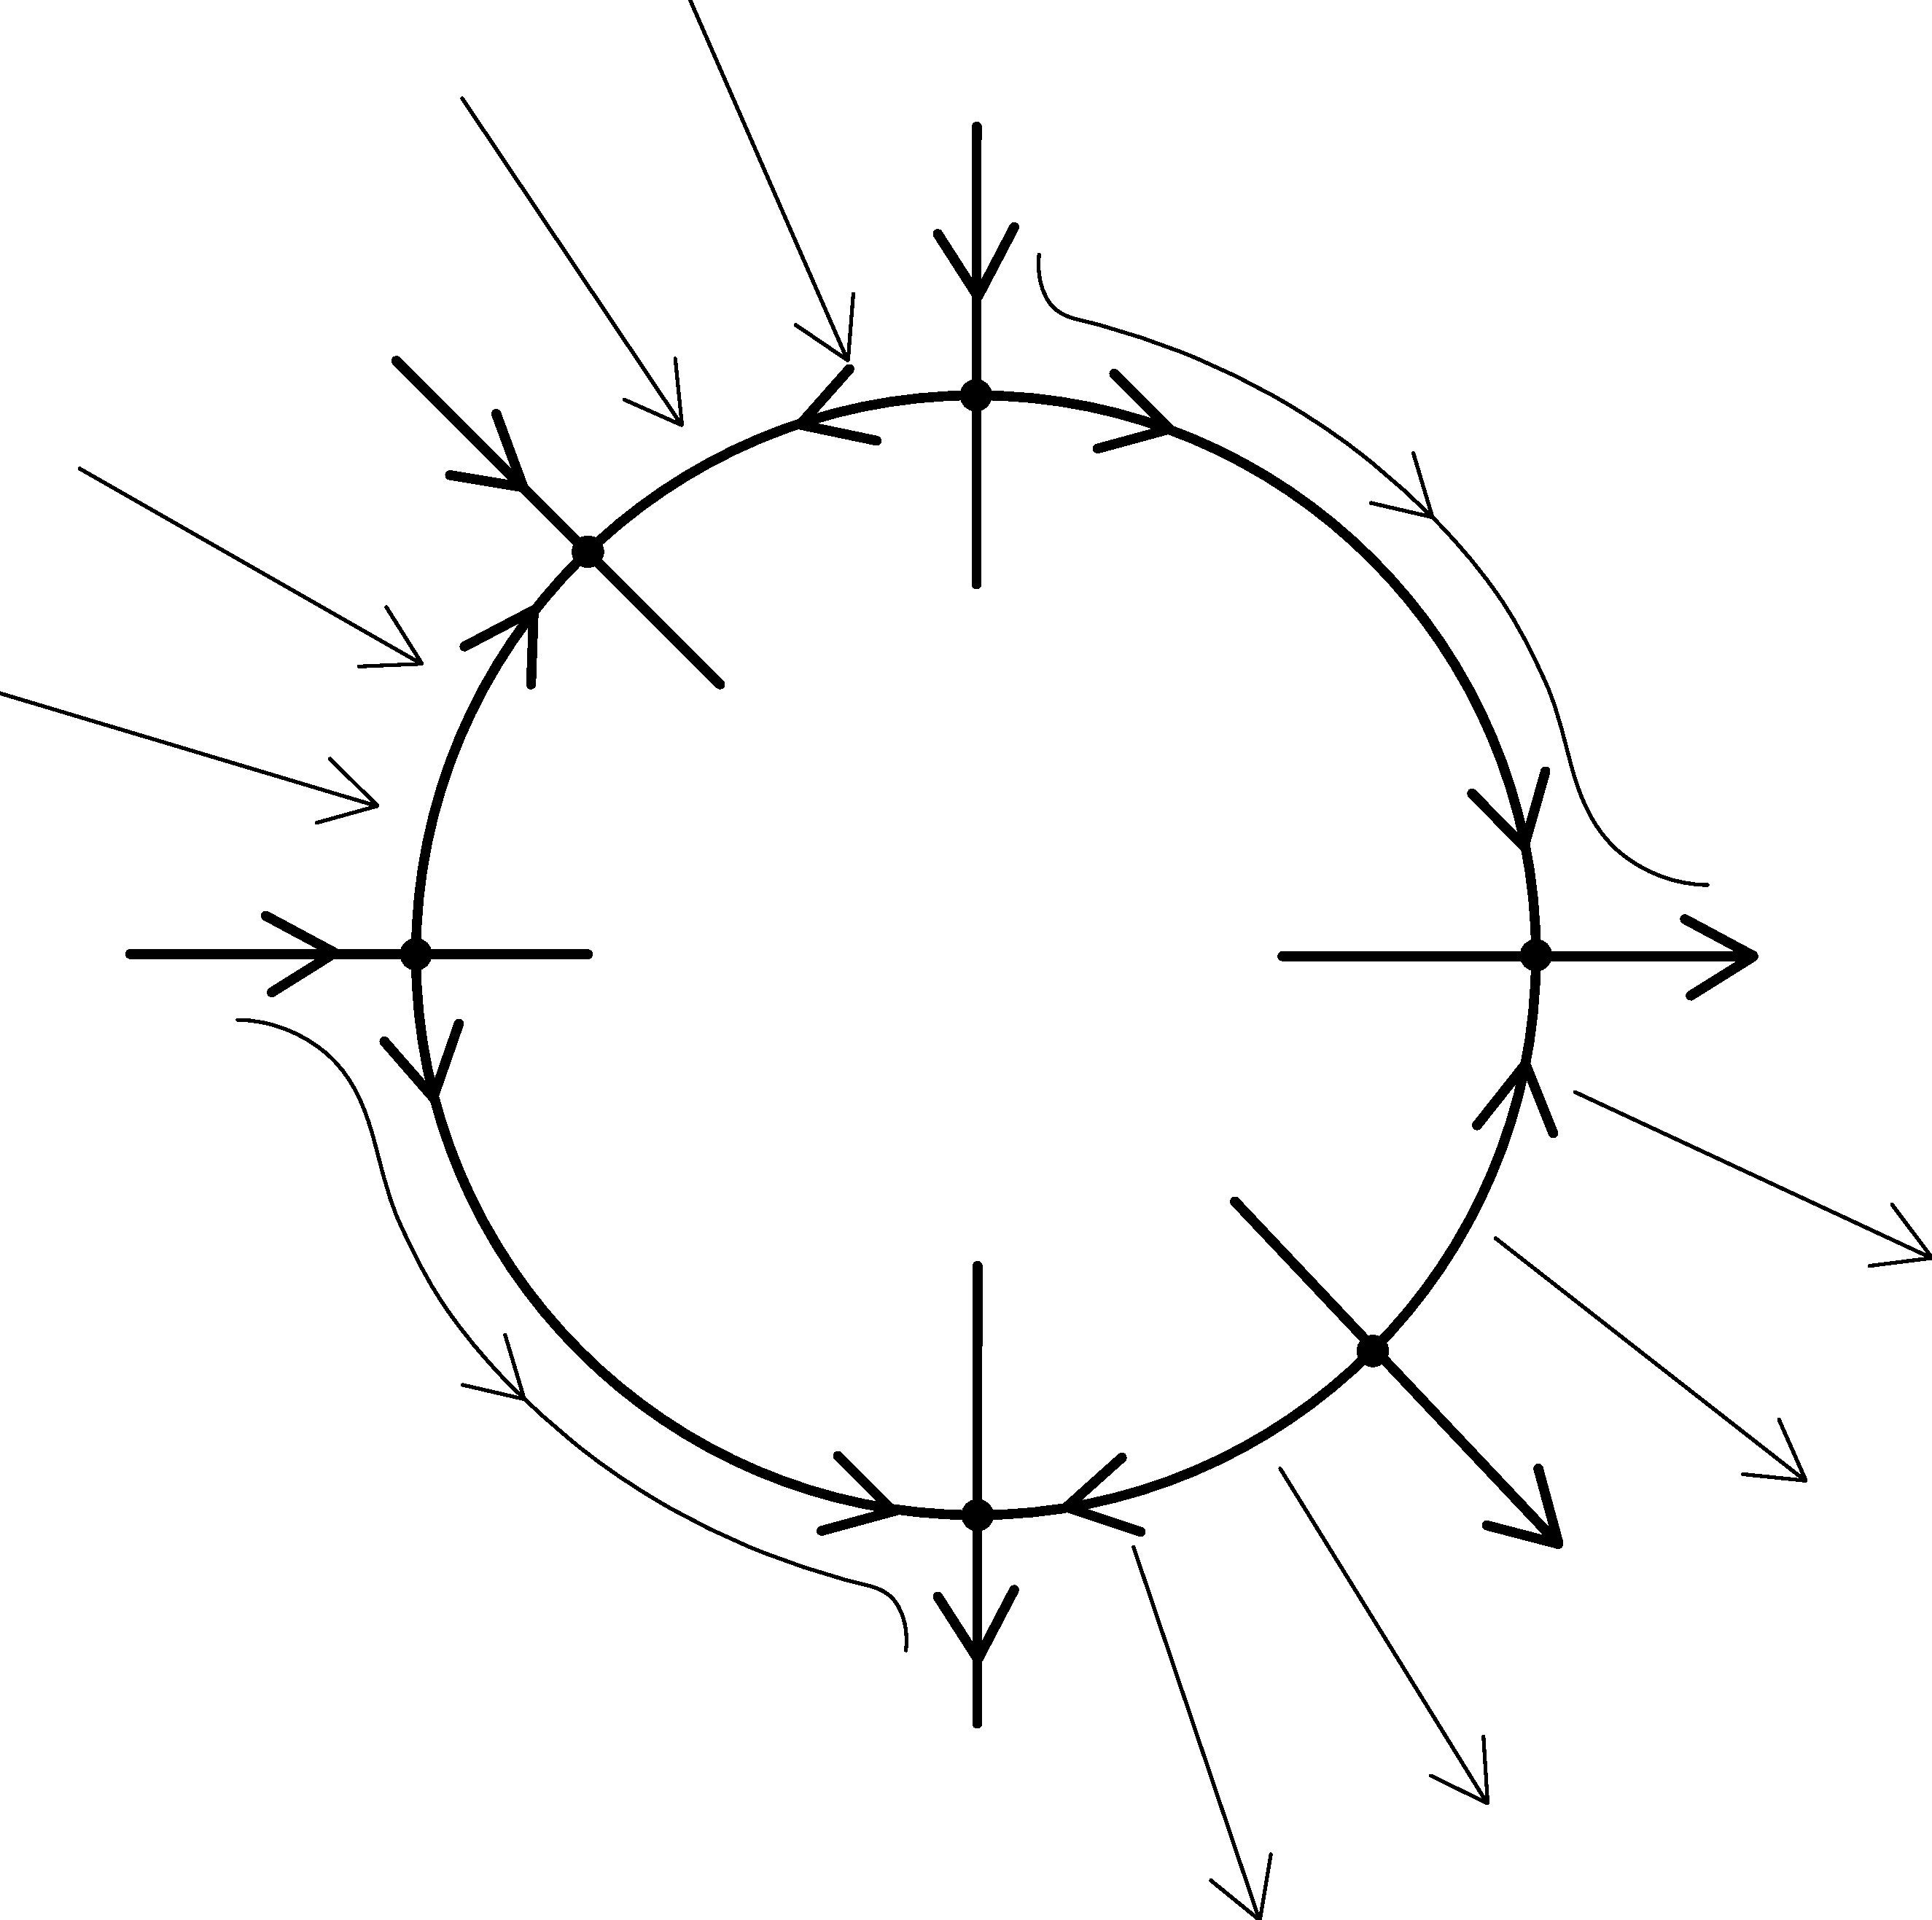
\includegraphics[width=\textwidth]{../img/blowingUpPolar(Bmen1).pdf}
			\caption{$B < 1$.}
		\end{subfigure}
		\hfill
		\begin{subfigure}{0.305\textwidth}
			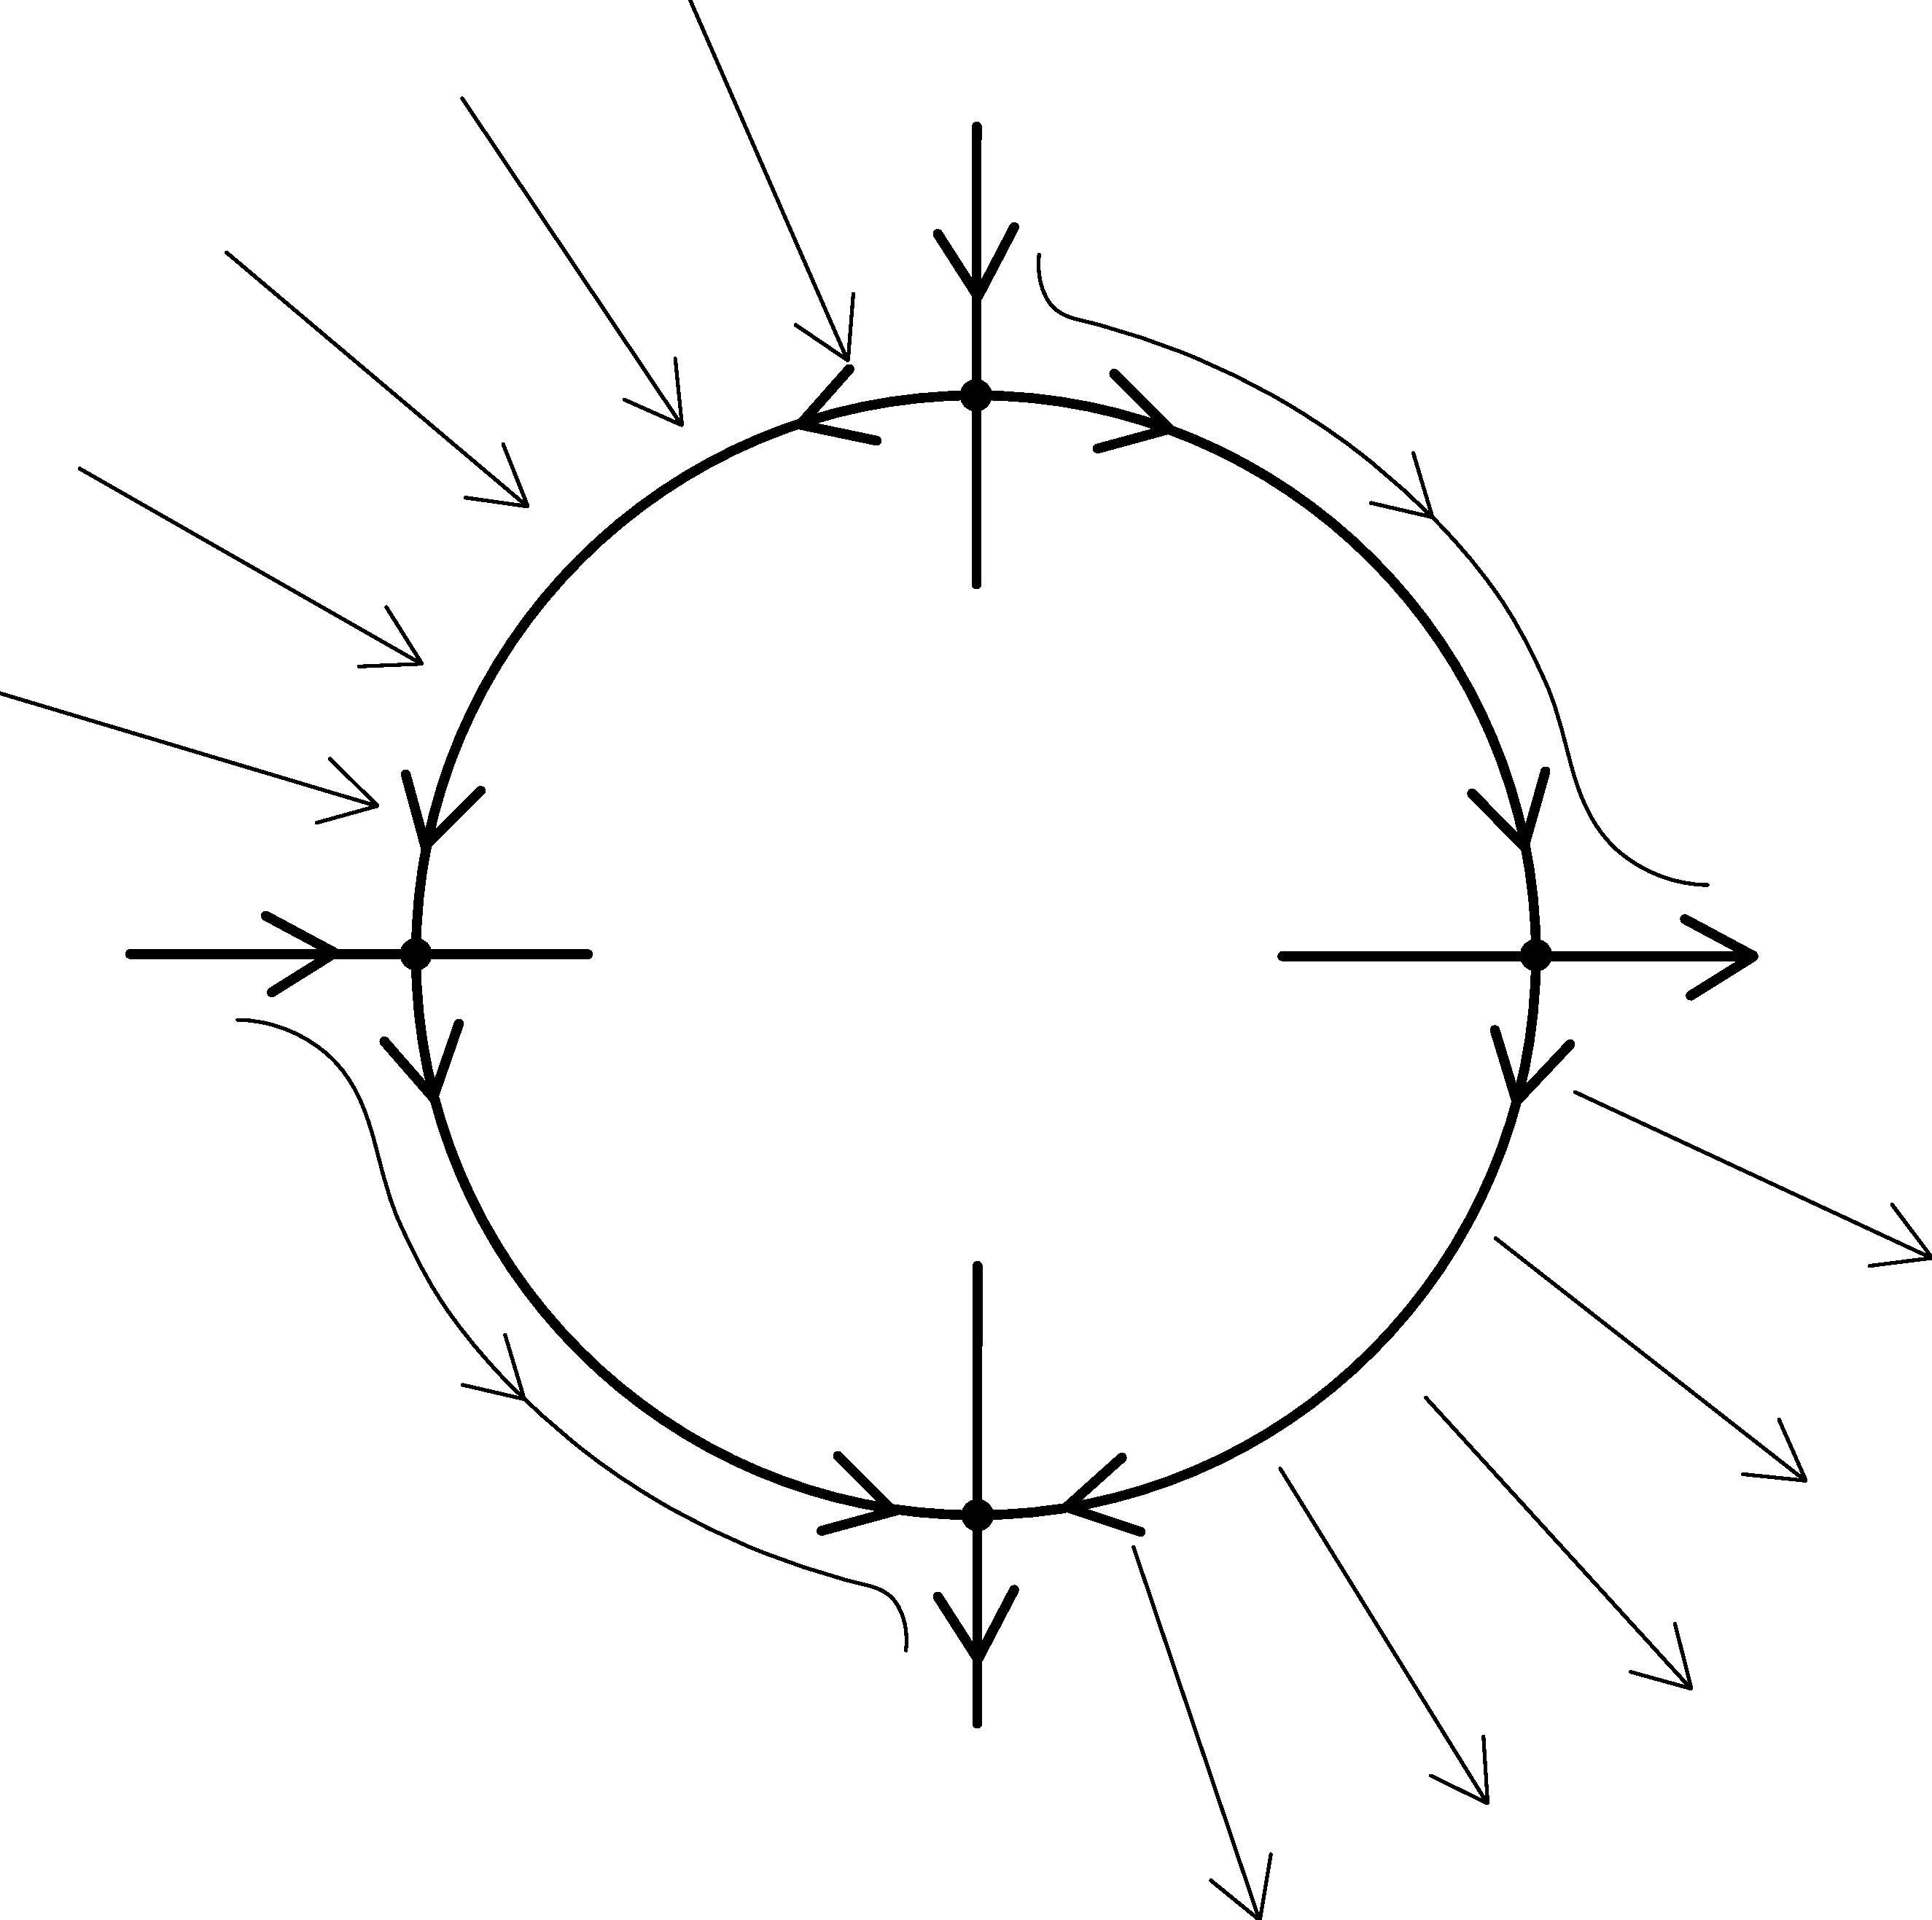
\includegraphics[width=\textwidth]{../img/blowingUpPolar(Bigu1).pdf}
			\caption{$B = 1$.}
		\end{subfigure}
		\hfill
		\begin{subfigure}{0.35\textwidth}
			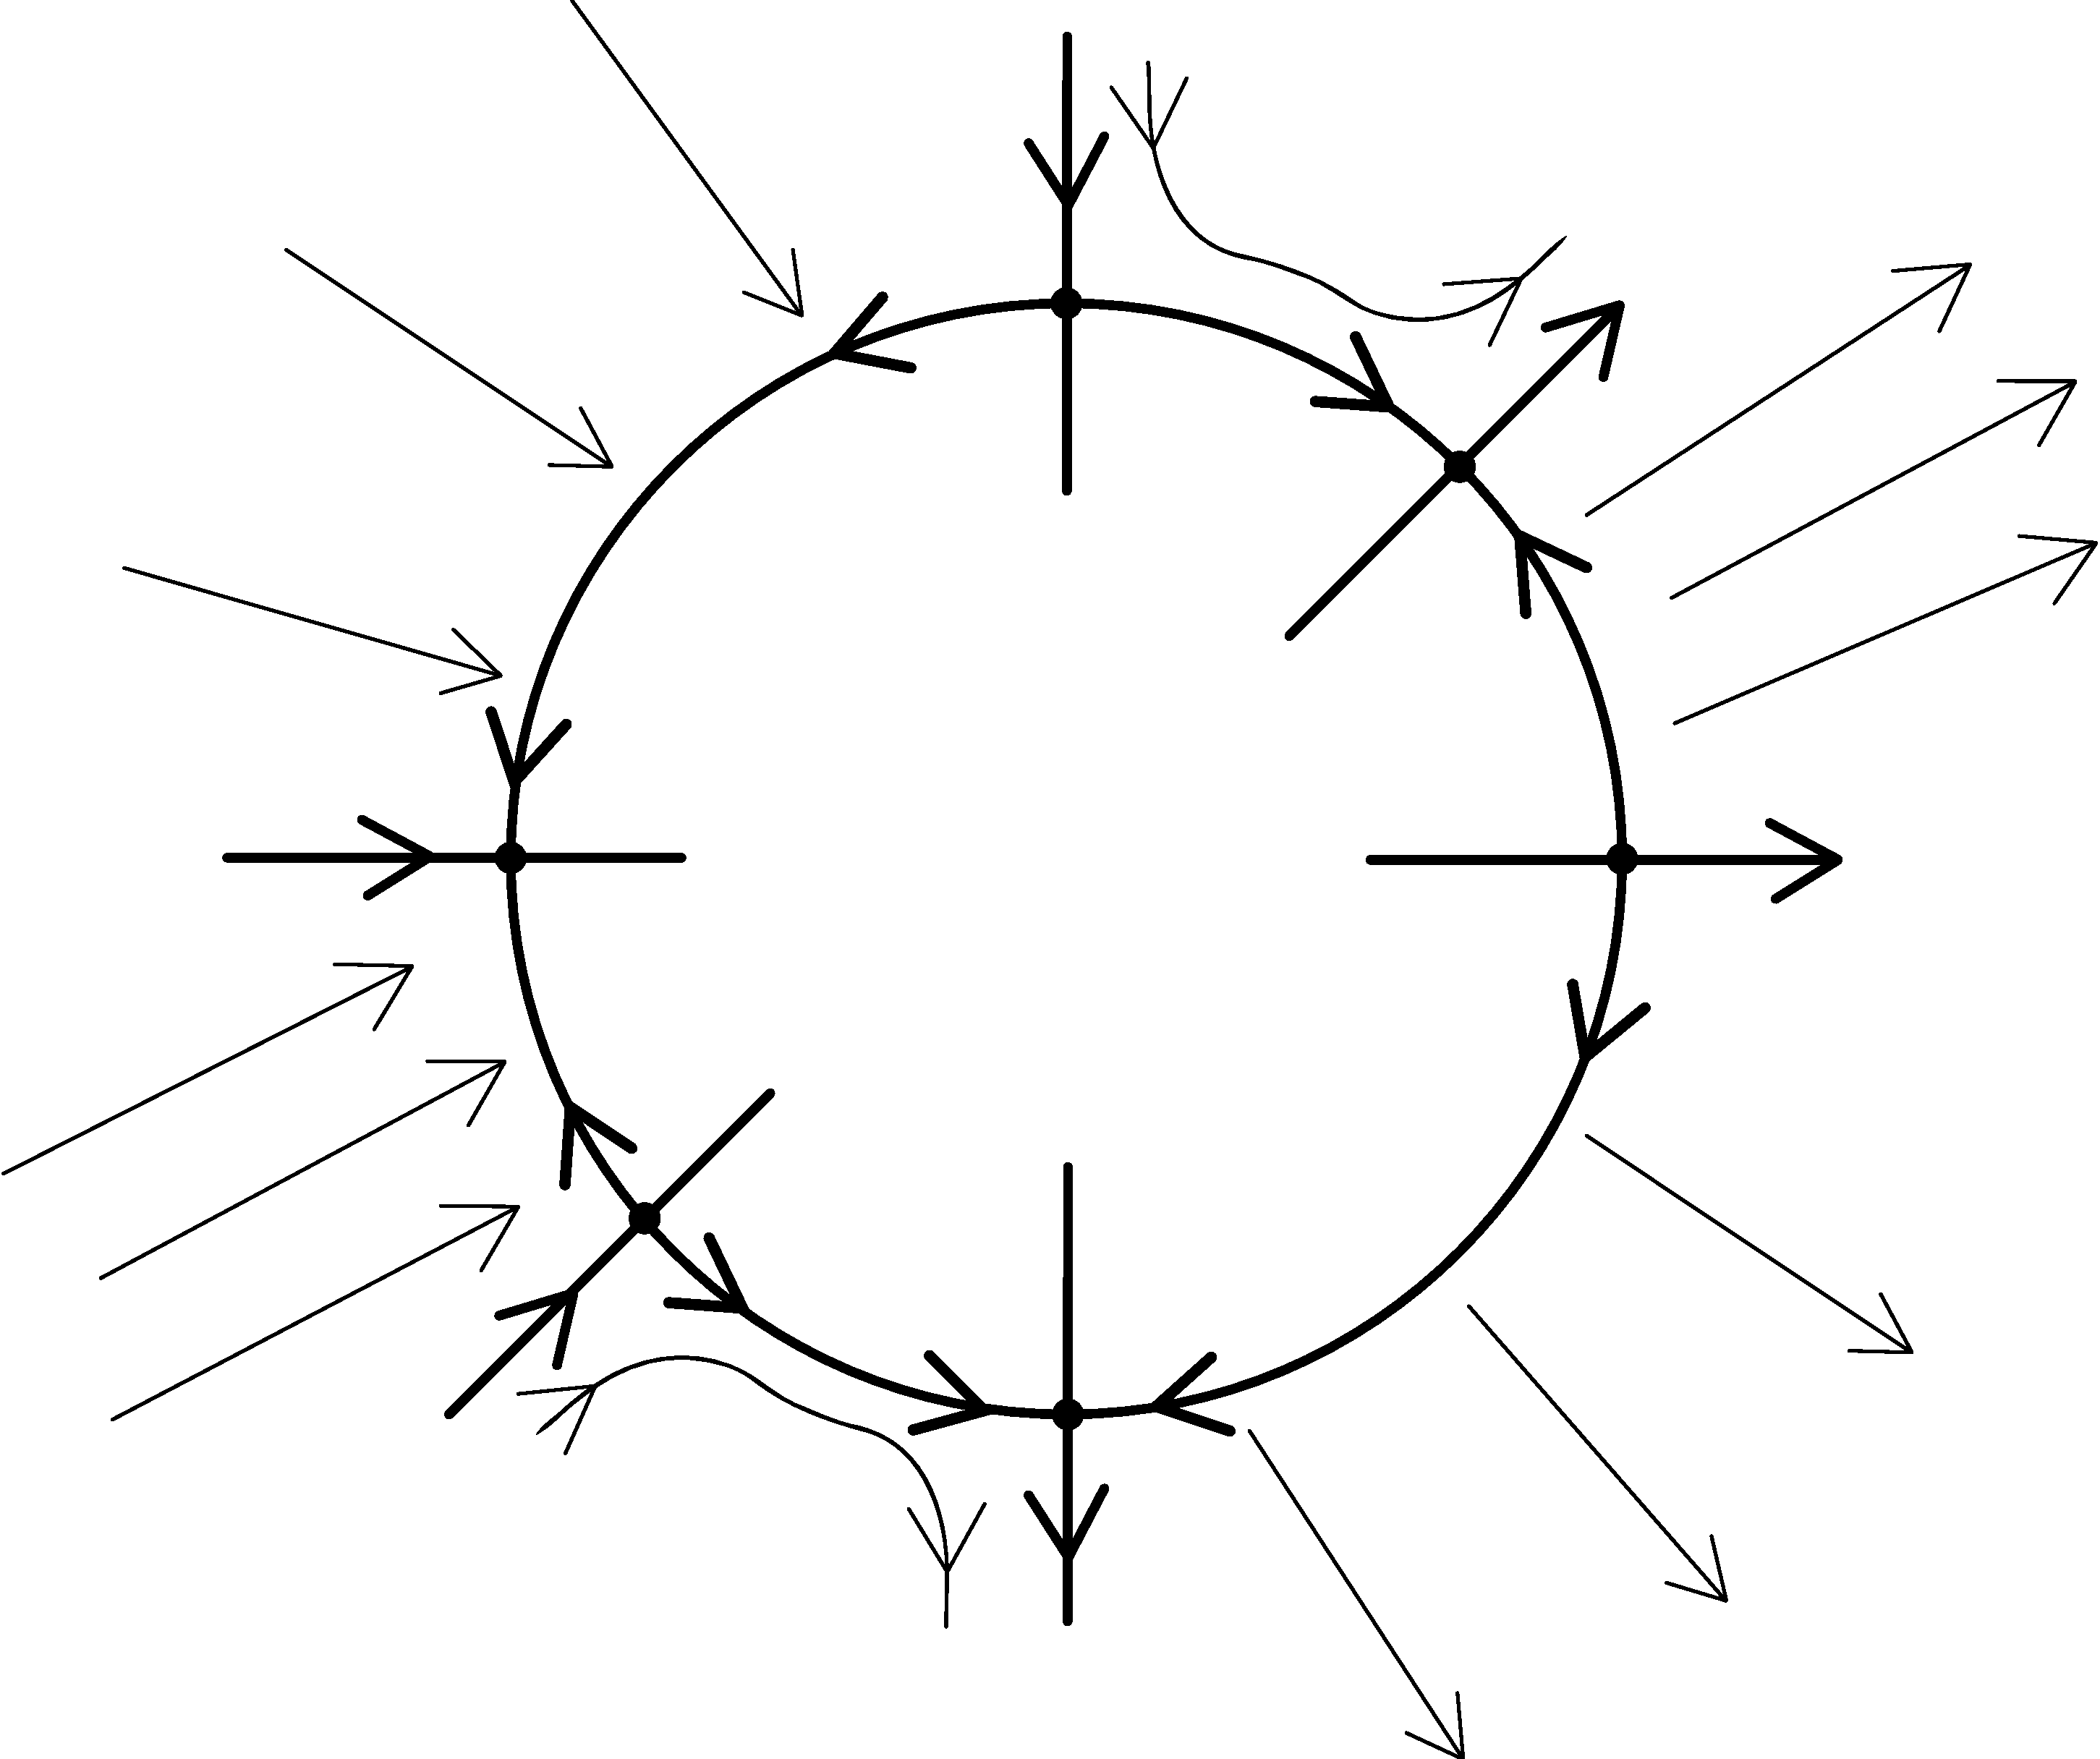
\includegraphics[width=\textwidth]{../img/blowingUpPolar(Bmay1).pdf}
			\caption{$B > 1$.}
		\end{subfigure}
		\caption{Blow-up en el origen del sistema \eqref{eq: modelo2} para diferentes valores de $B$.}
	\end{figure}
	
	\begin{theorem}
		Sean $$A_c = \sqrt{\dfrac{2H^3 + H^2(1 - H)\sqrt{3H(4 - H)}}{4-3H(3-H)}}, \; B_c(A) = \dfrac{H^2(1-2H) - A^2}{A^2 + H^2}<1,$$ $\Delta = (\operatorname{tr}(DY_\delta(H,H)))^2 - 4\det(DY_\delta(H,H))$ y $\mathcal{R} = \left\{ (H, A) \in (0, 1) \times (0, 1) \;\middle|\; H < \dfrac{1}{2}, \; A^2 < H^2(1 - 2H) \right\}$, para $(H, A) \in \mathcal{R}$ se tienen los siguientes casos:
		\begin{itemize}
			\item Si $B<B_c(A)$, entonces:
			\begin{itemize}
				\item si $\Delta<0$, el equilibrio $(H,H)$ es un foco inestable;
				\item si $\Delta=0$, $(H,H)$ es un nodo degenerado inestable;
				\item si $\Delta>0$, $(H,H)$ es un nodo inestable.
			\end{itemize}
			\item Si $B=B_c(A)$ y
			\begin{itemize}
				\item $H \in \left(0,(3 - \sqrt{6})/3 \right)$, entonces:
				\begin{itemize}
					\item si $A<A_c$, $l_1<0$ por lo que $(H,H)$ es un foco débil inestable rodeado por un ciclo límite estable;
					\item si $A=A_c$, $l_1=0$ y $l_2<0$ por lo que $(H,H)$ es un foco débil estable de segundo orden, rodeado por un ciclo límite inestable, el cual se encuentra contenido en el interior de un segundo ciclo límite estable;
					\item si $A>A_c$, $l_1>0$ por lo que $(H,H)$ es un foco débil estable rodeado por un ciclo límite inestable.
				\end{itemize}
				\item $H \in [(3 - \sqrt{6})/3, 1/2)$, entonces $l_1<0$ y $(H,H)$ es un foco débil inestable rodeado por un ciclo límite estable.
			\end{itemize}
			\item Si $B>B_c(A)$, entonces:
			\begin{itemize}
				\item si $\Delta<0$, el equilibrio $(H,H)$ es un foco estable;
				\item si $\Delta=0$, $(H,H)$ es un nodo degenerado estable;
				\item si $\Delta>0$, $(H,H)$ es un nodo estable.
			\end{itemize}
		\end{itemize}
		Para los valores $(H, A) \in (0, 1) \times (0, 1)$ que no estan en $\mathcal{R}$, se tiene que
		\begin{itemize}
			\item si $\Delta<0$, el equilibrio $(H,H)$ es un foco estable;
			\item si $\Delta=0$, $(H,H)$ es un nodo degenerado estable;
			\item si $\Delta>0$, $(H,H)$ es un nodo estable.
		\end{itemize}
		\label{teo: equilibrioH}
	\end{theorem}
	\begin{proof}
		Para estudiar la naturaleza del punto de equilibrio $(H,H)$ con $H \in (0,1)$, del Lema \autoref{lem: polinomio} tenemos que: $$Q=\dfrac{(1-H)(A^2+H^{2})}{H^{2}}.$$ Sustituyendo esta expresión en \eqref{eq: modelo2} se obtiene el nuevo sistema topológicamente equivalente:
		\begin{equation}
			Y_{\delta}:
			\begin{cases}
				\dfrac{du}{d \tau} = \left((1 - u)(u^{2} + A^{2}) - \dfrac{(1-H)(A^2+H^{2})}{H^{2}} u v\right)u^{2}, \\[5pt]
				\dfrac{dv}{d \tau} = B(u - v)(u^{2} + A^{2})v,
			\end{cases}
			\label{eq: modelo2.1}
		\end{equation}
		con $\delta = (A, B)$, cuya matriz jacobiana en el equilibrio $(H,H)$ está dada por:
		\begin{equation*}
			DY_\delta(H,H) =
			\begin{bmatrix}
				-H(H^{2}(2H-1)+A^2) & -H(1-H)(A^2+H^2) \\
				BH(A^{2}+H^{2}) & -BH(A^{2}+H^{2})
			\end{bmatrix},
		\end{equation*}
		con
		\begin{equation*}
			\begin{aligned}
				\operatorname{tr}(DY_\delta(H,H)) &= -H(B(A^2+H^2)+H^2(2H-1)+A^2), \\
				\det(DY_\delta(H,H)) &= BH^2(A^2+H^2)(H^3+A^2(2-H)) > 0.
			\end{aligned}
		\end{equation*}
		y valores propios $$\lambda_{1,2}(\delta) = \dfrac{\operatorname{tr}(DY_\delta(H,H)) \pm \sqrt{\Delta}}{2}.$$ La estabilidad del equilibrio $(H,H)$ estará determinada por el signo de la traza y del discriminante $\Delta$, para ello notemos que $\operatorname{tr}(DY_\delta(H,H))=0$ si, y solo si
		\begin{equation*}
			B = \dfrac{H^2(1-2H) - A^2}{A^2 + H^2} := B_c(A),
			\label{eq: Bcritico}
		\end{equation*}
		y puesto que $B>0$, $B_c(A)$ debe ser estrictamente positivo, esto se da bajo las restricciones: $H<1/2 \; \text{ y } \; A^2 < H^2(1-2H),$ donde $$B_c(A)=1-2\dfrac{A^2+H^3}{A^2+H^2}<1.$$ Así para $(H,A) \in \mathcal{R}$, $\operatorname{tr}(DY_\delta(H,H))<0$ si, y solo si $B<B_c$; los subcasos de estabilidad del equilibrio interior en este caso, al igual que para $B>B_c$, son resultados inmediatos determinados a partir de $\lambda_{1,2}(\delta)$ y del signo del discriminante $\Delta.$ \\
		
		Ahora, con el propósito de validar la estructura cualitativa para el caso $B = B_c$, calcularemos el primer número de Lyapunov. Para ello trasladamos el equilibrio $(H,H)$ al origen, sustituyendo $u = \bar{u} + H$ y $v = \bar{v} + H$ en el sistema $Y_\delta$. Además, reemplazamos el valor crítico $B_c$, obteniendo:
		\begin{equation*}
			Z_{\beta}:
			\begin{cases}
				\dfrac{d\bar{u}}{d \tau} = [(1 - \bar{u} - H)[(\bar{u} + H)^{2} + A^{2}] - \dfrac{(1-H)(A^2+H^{2})}{H^{2}} (\bar{u} + H) (\bar{v} + H)](\bar{u} + H)^{2}, \\[5pt]
				\dfrac{d\bar{v}}{d \tau} = \dfrac{H^2(1-2H) - A^2}{A^2 + H^2}(\bar{u} - \bar{v})[(\bar{u} + H)^{2} + A^{2}](\bar{v} + H),
			\end{cases}
		\end{equation*}
		donde $\beta = A$, $H<1/2 \; \text{ y } \; A^2 < H^2(1-2H).$ La matriz jacobiana evaluada en el origen está dada por
		\begin{equation*}
			DZ_{\beta}(0,0) =
			\begin{bmatrix}
				a & b \\
				a & - a
			\end{bmatrix},
		\end{equation*}
		con
		\begin{equation*}
			\begin{aligned}
				a &= H[H^{2}(1-2H)-A^2], \\
				b &= -H(1-H)(A^2+H^2).
			\end{aligned}
		\end{equation*}
		y valores propios complejos puros $\pm \omega = \sqrt{ad}$ donde $d = H[H^3+A^2(2-H)]$. Como el origen es un punto crítico del sistema o campo $Z_{\beta}$, este puede expresarse como
		\begin{equation}
			\left(\dfrac{d\bar{u}}{d \tau}, \dfrac{d\bar{v}}{d \tau}\right)^T=DZ_{\beta}(0,0)(\bar{v},\bar{v})^T+(F_1(\bar{v},\bar{v}), F_2(\bar{u},\bar{v}))^T,
			\label{eq: sistemal1}
		\end{equation}
		donde
		\begin{equation}
			\begin{aligned}
				F_1 = & -3\bar{u}\bar{v}(1 - H)(A^2 + H^2) \\
				& + \bar{u}^2\left(-2A^2 + (3 - 7H)H^2 + \dfrac{3b}{H^2} \bar{v} \right) \\ 
				& + \bar{u}^3\left(\dfrac{3(1 - 3H)H^2 - A^2}{H} + \dfrac{b}{H^3} \bar{v} \right) \\ 
				& + \bar{u}^4(1 - 5H) - \bar{u}^5, \\
				F_2 = & \; \bar{u} \left(\dfrac{a(A^2 - H^2)}{H(A^2 + H^2)} \bar{v} - \dfrac{2a}{A^2 + H^2} \bar{v}^2 \right) \\
				& + \bar{u}^2\left(\dfrac{2aH}{A^2 + H^2} + \dfrac{a}{A^2 + H^2} \bar{v} - \dfrac{a}{H(A^2 + H^2)} \bar{v}^2 \right) \\
				& + \bar{u}^3\left( \dfrac{a}{A^2 + H^2} + \dfrac{a}{H(A^2 + H^2)} \bar{v} \right) - \dfrac{a}{H} \bar{v}^2.
			\end{aligned}
			\label{eq: expansionF1,2}
		\end{equation}
		El primer coeficiente de Lyapunov estará dado por \cite{kuznetsov}[p.~110]
		\begin{equation}
			l_1 = \dfrac{1}{2 \omega^2}Re(i g_{20}g_{11} + \omega g_{21}),
			\label{eq: l1}
		\end{equation}
		donde las expresiones $ g_{20}, g_{11}$ y $g_{21}$ se determinan a partir de las igualdades
		\begin{equation*}
			g_{20}=G_{zz}, \; g_{11}=G_{zw}, \; g_{21}=G_{zzw},
		\end{equation*}
		con $G_{z z}, \;G_{z w}$ y $G_{z z w}$ dadas por las derivadas parciales evaluadas en $z=w=0$ de la función de variable compleja
		\begin{equation}
			G(z,w) = \bar{p_1}F_1(zq_1+w\bar{q_1}, zq_2+w\bar{q_2}) + \bar{p_2}F_2(zq_1+w\bar{q_1}, zq_2+w\bar{q_2}),
			\label{eq: funComplejaL1}
		\end{equation}
		donde
		\begin{equation}
			p = (p_1,p_2)^T =
			\begin{pmatrix}
				i/2m\\
				1/2 - i/2m
			\end{pmatrix}, \quad
			q = (q_1,q_2)^T =
			\begin{pmatrix}
				1+m \; i\\
				1
			\end{pmatrix},
			\label{eq: vecComplejos}
		\end{equation}
		con $m = \sqrt{d/a}$ y donde $p$, $q$ son los autovectores asociados a los valores propios complejos puros $\mp \omega i$, de $DZ_\beta(0,0)^T$ y $DZ_\beta(0,0)$, respectivamente; con $\langle p,q \rangle = 1$ considerando el producto interno $\langle \bar{m},\bar{n} \rangle = \bar{m}_1 \bar{n}_1 + \bar{m}_2 \bar{n}_2$.
		
		\noindent Tomando en cuenta lo anterior, tenemos que:
		\begin{equation}
			\begin{aligned}
				g_{20} = & \dfrac{i}{m}\{[A^2(1 - 3H) + 2H^2(3 - 5H)](m-i)^2 \\ 
				& + B_cm[A^2 + H^2(3 + 2mi)](m+i) - 3H^2Q(m-i)(m-2i) \}, \\
				g_{11} = & \dfrac{i}{m} \{A^2(3H-1)(1 + m^2) + H^2[10H(1 + m^2) + 6(Q-1) \\ 
				& + m^2(-6 + 2B_c - 2B_cmi + 3Q)]\}, \\
				g_{21} = & \dfrac{i}{m} \{3i[A^2 + 2H(5H-2)](m-i)^2(m+i) \\ 
				& + B_cHm(m+i)[3 + m(3m-4i)] \\ 
				& + 3QH(m-i)(4i + m + m^2i)\},
			\end{aligned}
			\label{eq: g_klModelo2}
		\end{equation}
		así, de \eqref{eq: l1}:
		\begin{equation}
			l_1 = \dfrac{2A^2(1 - H)([4 - 3H(3 - H)]A^4 -4H^3A^2 - (3 - H)H^5)}{(A^2 + H^2)[(H^3 + A^2(2 - H))(H^2(1 - 2H)- A^2)]^{3/2}},
			\label{eq: l1Kuznetsov}
		\end{equation}
		donde el signo de $l_1$ dependerá exclusivamente del signo de la expresión
		\begin{equation*}
			L_1 = [4 - 3H(3-H)]A^4 - 4H^3A^2 - (3-H)H^5,
		\end{equation*}
		con $4 - 3H(3-H) > 0$. El primer coeficiente de Lyapunov se anulará para:
		\begin{equation*}
			\begin{aligned}
				A^2 &= \dfrac{2H^3 + H^2(1 - H)\sqrt{3H(4 - H)}}{4-3H(3-H)} := A^2_c,
			\end{aligned}
		\end{equation*}
		$\forall H \in \left(0,(3 - \sqrt{6})/3 \right)$, esta restricción con el fin de que $A_c^2 < H^2(1-2H)$. Así para $A<A_c$, $L_1<0$ y $(H,H)$ es un foco débil inestable rodeado por un único ciclo límite estable. Similarmente para $A>A_c$, $L_1 > 0$ y $(H,H)$ es un foco débil estable rodeado por un ciclo límite inestable. Ahora, note que $\forall H \in [(3 - \sqrt{6})/3, 1/2)$, $A_c^2 \geq H^2(1-2H)$ por lo que $A<A_c, \; \forall A$ así $L_1<0$ y $(H,H)$ es un foco débil inestable rodeado por un ciclo límite estable, en este caso. \\
		
		\noindent Para poder determinar la estabilidad del equilibrio $(H,H)$ para el caso $A=A_c$, debemos calcular el segundo coeficiente de lyapunov. Procedemos a reemplazar el valor paramétrico $A=A_c$ en el sistema \eqref{eq: sistemal1}, obteniendo:
		\begin{equation}
			W:
			\begin{cases}
				\dfrac{d\bar{u}}{d \tau} = \bar{a}\bar{u} + \bar{b}\bar{v} + F_1(\bar{u}, \bar{v}), \\[5pt]
				\dfrac{d\bar{v}}{d \tau} = \bar{a}\bar{u} - \bar{a}\bar{v} + F_2(\bar{u}, \bar{v}),
			\end{cases}
			\label{eq: normalFormWn}
		\end{equation}
		con $F_{1}$ y $F_2$ dadas por las expansiones \eqref{eq: expansionF1,2}, sustituyendo $A=A_c$ y
		\begin{equation*}
			\begin{aligned}
				\bar{a} &= \dfrac{H^3(1 - H)[4 - 3H(5 - 2H) - \sqrt{3H(4 - H)}]}{4 - 3H(3 - H)}, \\
				\bar{b} &= -\dfrac{H^3(1 - H)^2[4 - 3H + \sqrt{3H(4 - H)}]}{4 - 3H(3 - H)}.
			\end{aligned}
		\end{equation*}
		El segundo coeficiente de Lyapunov está dado por \cite{kuznetsov}[p.~344]
		\begin{equation}
			\begin{aligned}
				12l_2 = {} & \dfrac{1}{\omega} \text{Re } g_{32} \\
				& + \dfrac{1}{\omega^2} \text{Im } \left[ g_{20} \bar{g}_{31} - g_{11} (4 g_{31} + 3 \bar{g}_{22}) - \dfrac{1}{3} g_{02} (g_{40} + \bar{g}_{13}) - g_{30} g_{12} \right] \\
				& + \dfrac{1}{\omega^3} \left\{ \text{Re } \left[ g_{20} \left( \bar{g}_{11} (3 g_{12} - \bar{g}_{30}) + g_{02} \left( \bar{g}_{12} - \dfrac{1}{3} g_{30} \right) + \dfrac{1}{3} \bar{g}_{02} g_{03} \right) \right.\right. \\
				& \qquad\qquad\qquad \left. + g_{11} \left( \bar{g}_{02} \left( \dfrac{5}{3} \bar{g}_{30} + 3 g_{12} \right) + \dfrac{1}{3} g_{02} \bar{g}_{03} - 4 g_{11} g_{30} \right) \right] \\
				& \qquad\qquad \left. + \, 3 \text{ Im}(g_{20} g_{11}) \text{ Im } g_{21} \right\} \\
				& + \dfrac{1}{\omega^4} \left\{ \text{Im} \left[ g_{11} \bar{g}_{02} \left( \bar{g}_{20}^2 - 3 \bar{g}_{20} g_{11} - 4 g_{11}^2 \right) \right] \right. \\
				& \qquad\qquad \left. + \, \text{Im}(g_{20} g_{11}) \left[ 3 \text{ Re}(g_{20} g_{11}) - 2 |g_{02}|^2 \right] \right\},
			\end{aligned}
			\label{eq: l2}
		\end{equation}
		con $\omega = \sqrt{\bar{a}\bar{d}}$, donde $\bar{d} = H^4+\dfrac{H^3(2-H) [2H+(1-H) \sqrt{3H(4-H)}]}{4-3H(3-H)}$ y las expresiones $g_{kl}$ estarán dadas por $g_{kl}=G_{z w}$ que representan las derivadas parciales de la función de variable compleja \eqref{eq: funComplejaL1} evaluadas en $z=w=0$ con $p_1, p_2, q_1, q_2$ dadas por \eqref{eq: vecComplejos} reemplazando $m$ por $\bar{m} = \sqrt{\bar{d}/\bar{a}}$, donde por ejemplo $g_{02}=G_{ww}$, $g_{31}=G_{zzzw}$, de manera similar se determinan las demás expresiones. Los términos $g_{20}, \; g_{11}, \; \text{y } g_{21}$ son dados por \eqref{eq: g_klModelo2} remplazando $A=A_c$ y $m = \bar{m}$, además
		\begin{equation*}
			\begin{aligned}
				g_{31} = & \dfrac{i}{\bar{m}} \{6(\bar{m}^2+1)[-2 + (B_c-4)\bar{m}i + (B_c+2)\bar{m}^2 \\
				& - 10H(\bar{m}-i)^2] - 6Q(\bar{m}^3 + 3\bar{m} -2i)\}, \\
				g_{32} = & \dfrac{-60}{\bar{m}}(\bar{m}-i)^3 (\bar{m}+i)^2, \\
				g_{22} = & \dfrac{2i}{\bar{m}} [4B_c\bar{m}^2(1 - \bar{m}i) + 6(5H-1)(\bar{m}^2+1)^2 + 6Q(\bar{m}^2+1)], \\
				g_{02} = & \dfrac{-(\bar{m}+i)}{\bar{m}}\{ A_c^2[1 - 3H + (B_c + 3H - 1)\bar{m}i] \\
				& + H^2[6 + 2B_c\bar{m}^2 + 10Hi(\bar{m}+i) - 6Q + 3\bar{m}i(B_c + Q - 2)] \}, \\
				g_{40} = & \dfrac{12i}{\bar{m}} \{ 5H(\bar{m}-i)^4 - (\bar{m}-i)^2[-1 + (B_c+1)\bar{m}^2 \\
				& + Q + (B_c + Q - 2)\bar{m}i] \}, \\
				g_{13} = & \dfrac{-6i}{\bar{m}} (\bar{m}+i)^2[-2 + 10H - B_c\bar{m}i \\
				& + \bar{m}^2(B_c + 10H-2) + Q(\bar{m}i+2)], \\
				g_{30} = & \dfrac{3}{\bar{m}} \{ [A_c^2 + 2H(5H-2)](\bar{m}-i)^3 \\
				& + B_cH\bar{m}(1 - \bar{m}i)[\bar{m}(\bar{m}-4i)-3] + HQ(\bar{m}-i)^2(\bar{m}-4i) \},
			\end{aligned}
		\end{equation*}
		\begin{equation*}
			\begin{aligned}
				g_{12} = & \dfrac{\bar{m}+i}{\bar{m}} \{3A_c^2(\bar{m}^2+1) + H[30H(\bar{m}^2+1)\\
				& + \bar{m}[B_c(-3i + \bar{m}(4 - 3\bar{m}i)) + 3\bar{m}(Q-4) + 3Qi] + 12(Q-1)]\}, \\
				g_{03} = & \dfrac{-3(\bar{m}+i)^2}{\bar{m}} \{A_c^2(\bar{m}+i) \\
				& + H\left[10H(\bar{m}+i) + 4i(Q-1) + \bar{m}(B_c(3 - \bar{m}i) + Q -4)\right]\},
			\end{aligned}
		\end{equation*}
		donde
		\begin{equation*}
			\begin{aligned}
				B_c &= \dfrac{2-3H - \sqrt{3H(4 - H)}}{2}, \\
				Q &= H^2 \dfrac{H[2-3(3-H)]+(1-H)\sqrt{3H(4-H)}+4}{4-3H(3-H)}.
			\end{aligned}
		\end{equation*}
		Tomando en cuenta lo anterior computamos $l_2$ dada en \eqref{eq: l2}. El cálculo numérico de $l_2$ arroja que para cualquier valor $H \in \left(0,(3 - \sqrt{6})/3 \right)$, $l_2<0$; por lo tanto, el punto crítico $(H,H)$ es un foco débil estable de segundo orden, rodeado por un ciclo límite inestable y este a su vez, por un ciclo límite estable.
		\begin{table}[H]
			\centering
			\caption{Algúnos valores de $l_2$ para $H \in \left(0,(3 - \sqrt{6})/3 \right)$.}
			\label{tab: ejemplosL2}
			
			\begin{tabular}{ccccl}
				\hline
				$H$ & $A_c$ & $B_c$ & $Q$ & $l_2$ \\
				\hline
				0.0247 & 0.0096 & 0.6918 & 1.1246 & -1021240 \\
				0.0645 & 0.0338 & 0.4671 & 1.1932 & -100399 \\
				0.0646 & 0.0339 & 0.4664 & 1.1933 & -100023 \\
				0.0900 & 0.0530 & 0.3511 & 1.2257 & -63026.4 \\
				0.0922 & 0.0548 & 0.3418 & 1.2283 & -61890.6 \\
				0.0953 & 0.0573 & 0.3289 & 1.2319 & -60651.6 \\
				0.1529 & 0.1114 & 0.1065 & 1.2971 & -180304 \\
				0.1633 & 0.1227 & 0.0694 & 1.3091 & -409538 \\
				0.1717 & 0.1321 & 0.0404 & 1.3190 & -1314910 \\
				0.1720 & 0.1325 & 0.0392 & 1.3194 & -1402770 \\
				\hline
			\end{tabular}
		\end{table}
		
		\noindent Por último, para los valores $(H, A) \in (0, 1) \times (0, 1)$ que no estan en $\mathcal{R}$, es decir, para $H \geq 1/2$ o $A^2 \geq H^2(1-2H)$ se tiene que $\operatorname{tr}(DY_\delta(H,H)) < 0$, por lo que $(H, H)$ es un atractor, los subcasos son determinados a partir del signo del discriminante $\Delta$.
	\end{proof}
	
	\begin{theorem}
		Una bifurcación de Hopf ocurre en el equilibrio $(H, H)$ para el valor de bifurcación $B = B_c$ y $A\neq A_c$.
		\label{teo: BifHopf}
	\end{theorem}
	\begin{proof}
		Del sistema \eqref{eq: modelo2.1}, por el \autoref{teo: equilibrioH} para $A\neq A_c$, $l_1 \neq 0$; así, para que ocurra una bifurcación de Hopf se deben satisfacer la condición espectral y la de transversalidad. Por el \autoref{teo: equilibrioH}, $DY_\delta(H,H)$ para $B = B_c$, posee un par de autovalores imaginarios puros $\lambda_1, \; \lambda_2 = \pm \sqrt{\det (DY_\delta(H,H))} \; i$, satisfaciendo así la condición espectral. Por otra parte, la velocidad de cruce de la parte real de los autovalores respecto al parámetro de bifurcación $B$, debe ser distinta de cero en el punto crítico, esto es:
		\begin{equation*}
			\begin{aligned}
				\left. \dfrac{d}{dB}(Re(\lambda(\delta))) \right|_{B=B_c} &= \left. \dfrac{d}{dB}\left(\dfrac{\operatorname{tr}(DY_\delta(H,H))}{2}\right) \right|_{B=B_c} \\
				&= -\dfrac{1}{2}H(A^{2}+H^{2}) \neq 0.
			\end{aligned}
		\end{equation*}
		Cumpliendo así las condiciones para que una bifurcación de Hopf ocurra en el sistema \eqref{eq: modelo2.1} para $B = B_c$ y $A\neq A_c$. Es claro que, esto también ocurrirá en el sistema \eqref{eq: modelo2} puesto que es topológicamente equivalente con el sistema \eqref{eq: modelo2.1}.
	\end{proof}
	
	\begin{figure}
		\centering
		\begin{subfigure}{0.49\textwidth}
			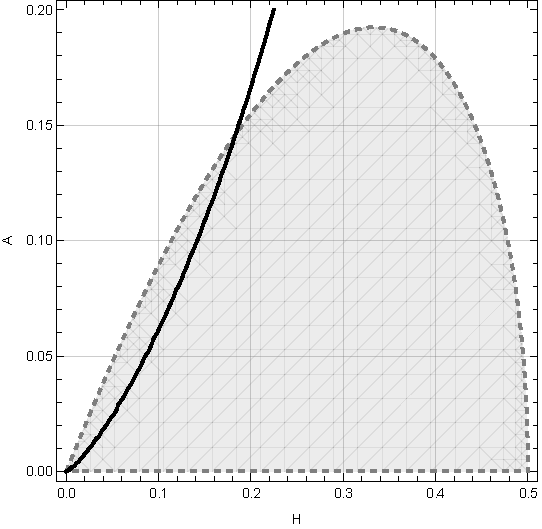
\includegraphics[width=1\textwidth]{../img/CurvaLyapunovAH.pdf}
			\caption{Curva $L_1 = 0$ y la región $\mathcal{R}$.}
			\label{fig: curvaL_1AH}
		\end{subfigure}
		\hfill
		\begin{subfigure}{0.49\textwidth}
			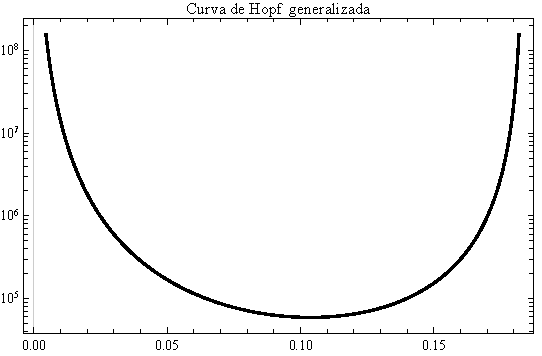
\includegraphics[width=1\textwidth]{../img/CurvaLyapunov2H.pdf}
			\caption{Curva $-l_2$ en escala logarítmica, dentro del dominio biológicamente relevante $0 < H < (3 - \sqrt{6})/3$.}
		\end{subfigure}
		\caption{Simulación numérica del primer ($l_1$) y segundo coeficiente de Lyapunov ($-l_2$).}
		\label{fig: simulacionNumericaL1L2}
	\end{figure}
	
	\begin{remark}
		
		La curva $L_1 = 0$ y la región de restricciones del sistema $\mathcal{R}$, puede observarse en la \autoref{fig: curvaL_1AH}. El modelo contará con una bifurcación de Hopf subcrítica ($l_1 > 0$) para los valores de $A$ y $H$ que se encuentren por encima de esta curva y dentro de la región restrictiva; de manera análoga, el sistema poseerá una bifurcación de Hopf supercrítica ($l_1 < 0$) para los valores que se encuentren debajo de esta curva y dentro de la región dada por las restricciones del sistema.
	\end{remark}
	
	\begin{theorem}
		Una bifurcación de Hopf generalizada (Bautin) ocurre en el equilibrio $(H, H)$ para el valor de bifurcación $\delta_0=(A_c, B_c)$.
	\end{theorem}
	\begin{proof}
		Considere el sistema \eqref{eq: modelo2.1}, por el \autoref{teo: equilibrioH} para $A = A_c$, $l_1 = 0$ y $l_2 \neq 0$; así, para que ocurra una bifurcación de Bautín se deben satisfacer la condición espectral y la de transversalidad. Por el \autoref{teo: BifHopf} la condición espectral se cumple. Por otra parte, el mapeo $\delta = (A,B) \longmapsto \left(Re(\lambda(\delta)), l_1(\delta)\right)$ debe ser regular en $\delta=\delta_0$, es decir
		\begin{equation*}
			\det \left. \begin{pmatrix}
				\dfrac{\partial Re(\lambda(\delta))}{\partial A} & \dfrac{\partial Re(\lambda(\delta))}{\partial B} \\[6pt]
				\dfrac{\partial l_1(\delta)}{\partial A} & \dfrac{\partial l_1(\delta)}{\partial B} 
			\end{pmatrix} \right|_{\delta=\delta_0} \neq 0,
		\end{equation*}
		esto es
		\begin{equation}
			\left. - \dfrac{\partial Re(\lambda(\delta))}{\partial B} \left( \dfrac{\partial l_1(\delta)}{\partial A} - \dfrac{\dfrac{\partial Re(\lambda(\delta))}{\partial A}}{\dfrac{\partial Re(\lambda(\delta))}{\partial B}} \dfrac{\partial l_1(\delta)}{\partial B} \right) \right|_{\delta=\delta_0} \neq 0.
			\label{eq: regularidadBautin}
		\end{equation}
		Como $Re(\lambda(\delta_0))=0$ y del \autoref{teo: BifHopf} sabemos que  $\left. \dfrac{\partial Re(\lambda(\delta))}{\partial B} \right|_{\delta=\delta_0} \neq 0$, por el teorema de la función implícita existe una función diferenciable $\phi(A)=B$ con dominio en una vecindad $V$ de $A_c$ tal que
		\begin{equation}
			\dfrac{dB}{dA}=\phi'(A)= - \dfrac{\dfrac{\partial Re(\lambda(\delta))}{\partial A}}{\dfrac{\partial Re(\lambda(\delta))}{\partial B}}, \; A \in V.
			\label{eq: teoFunImpli}
		\end{equation}
		Considerando lo anterior, por la regla de la cadena $$\dfrac{d l_1(A, \phi(A))}{dA} = \dfrac{\partial l_1(A, \phi(A))}{\partial A} + \phi'(A) \dfrac{\partial l_1(A, \phi(A))}{\partial \phi(A)},$$ así por lo anterior y por \eqref{eq: teoFunImpli} para una vecindad $V$ de $A_c$ la regularidad \eqref{eq: regularidadBautin} se reduce a probar que $$\left. \dfrac{d l_1(A, \phi(A))}{dA} \right|_{A=A_c} \neq 0.$$ Ahora, nótese que la función $\phi(A)$ está dada simplemente por $B_c(A)$ obtenida en \eqref{eq: Bcritico}, por lo que basta mostrar que la derivada con respecto a $A$ de $l_1$ determinada en \eqref{eq: l1Kuznetsov}, no se anula para $A=A_c$. Con este objetivo, considerando
		\begin{equation*}
			\begin{aligned}
				N &= 2A^2(1 - H)([4 - 3H(3 - H)]A^4 -4H^3A^2 - (3 - H)H^5) ,\\
				I &= (H^3 + A^2(2 - H))(H^2(1 - 2H)- A^2),
			\end{aligned}
		\end{equation*}
		de \eqref{eq: l1Kuznetsov} tenemos que $$l_1 = \dfrac{N}{(A^2+H^2)I^{3/2}},$$ asi
		\begin{equation}
			\dfrac{dl_1}{dA} = \dfrac{N' (A^2+H^2) I^{3/2} - N \left[2AI^{3/2} + (3/2)(A^2+H^2) I^{1/2} I' \right]}{(A^2+H^2)^2 I^3},
		\end{equation}
		por las restricciones del sistema $(A^2+H^2) I^{3/2} > 0$ y como $N=0$ en $A=A_c$ tenemos que $\left. \dfrac{d l_1}{dA} \right|_{A=A_c} \neq 0$ si, y solo si $N' \neq 0$ para $A=A_c$. Ahora el signo de
		\begin{equation*}
			N'= 4A(1-H) \left(3[4-3H(3-H)]A^4-8H^3A^2-(3-H)H^5\right)
		\end{equation*}
		estará determinado por la expresión $$3[4-3H(3-H)]A^4-8H^3A^2-(3-H)H^5,$$ la cual se anulará para
		\begin{equation*}
			\begin{aligned}
				A^2 &= \dfrac{8H^3 \pm \sqrt{64 H^6 + 12[4 - 3H(3-H)] (3-H)H^5}}{6[4-3H(3-H)]} \\
				&= \dfrac{1}{3} \dfrac{4H^3 + H^2\sqrt{36H - H^2[77 - 9H(6 - H)]}}{4-3H(3-H)} \neq A^2_c.
			\end{aligned}
		\end{equation*}
		Cumpliéndose así la condiciones necesarias para la bifurcación de Hopf generalizada en el sistema \eqref{eq: modelo2.1} para $\delta=\delta_0$. Es claro que, esto también ocurrirá en el sistema \eqref{eq: modelo2} puesto que es topológicamente equivalente con el sistema \eqref{eq: modelo2.1}.
	\end{proof}
	
\section{Discusión y trabajos a futuro}

En este trabajo se realizó un análisis cualitativo y local de un modelo depredador--presa tipo Leslie-Gower con respuesta funcional de Holling tipo III, propuesto originalmente por Gonzáles-Olivares et al.~\cite{articulo}. Mediante un cambio de variables y un reescalamiento temporal, realizado con el propósito de facilitar el análisis, se obtuvo un sistema topológicamente equivalente al modelo original. Esta transformación permitió, además, incorporar el origen al dominio de estudio y analizar su comportamiento local, aspecto que no era posible estudiar directamente en el sistema original.

A partir del estudio cualitativo del sistema polinomial de quinto orden obtenido, se establecieron los siguientes resultados:

\begin{enumerate}[leftmargin=*]
	\item Se determinó que el cuadrado unitario $\Gamma = \{ (u, v) \in \mathbb{R}^{2} \; | \; 0 \leq u \leq 1, \; 0 \leq v \leq 1 \} \subset \tilde{\Omega}$, es una región positivamente invariante. En consecuencia, toda solución que inicia en $\Gamma$ permanece en esta región para todo tiempo futuro, por lo que las soluciones biológicamente relevantes son acotadas, lo que demuestra que el modelo Leslie-Gower modificado está bien planteado. El difeomorfismo empleado para establecer la equivalencia topológica entre el sistema original y el sistema polinomial \eqref{eq: modelo2} permite restringir el análisis biológicamente relevante del modelo transformado a esta región $\Gamma$. En efecto, las sustituciones $u=\dfrac{x}{K}, \; v=\dfrac{y}{nK}$, normalizan las densidades poblacionales con respecto a las capacidades de carga asociadas a la presa y al depredador. De esta manera, los valores $u=1$ y $v=1$ representan, respectivamente, los niveles de población asociados a dichas capacidades de carga. Por tanto, el estudio de la dinámica dentro del cuadrado unitario $\Gamma$ resulta particularmente relevante desde el punto de vista biológico.
	
	\item Se obtuvieron tres puntos de equilibrio biológicamente relevantes: $(0,0), \; (1,0), \; \text{y} \; (H,H)$, donde $H\in(0,1)$ está determinado por la intersección de las isoclinas $v = \dfrac{(1-u)(u^2 + A^2)}{Q u}$ y $u=v$.
	
	\item Se clasificó el punto de equilibrio $(1,0)$ como un punto silla, independientemente de los valores de los parámetros del sistema.
	
	\begin{figure}[H]
		\centering
		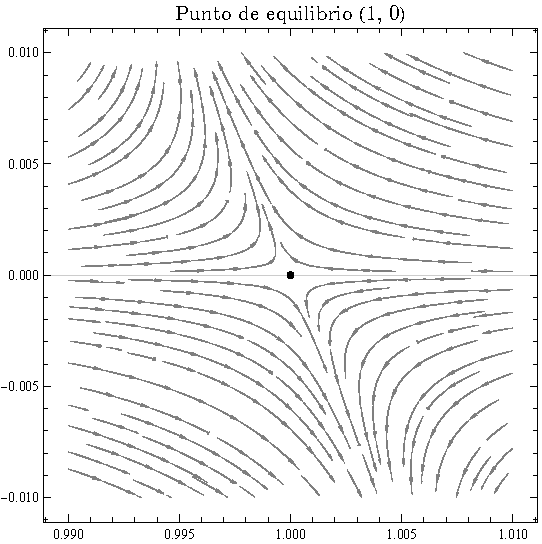
\includegraphics[width=.4\textwidth]{../img/puntoDeEquilibrio(1,0).pdf}
		\caption{Punto de equilibrio $(1, 0)$ para valores paramétricos aleatorios.}
	\end{figure}
	
	\item Se demostró que el punto de equilibrio $(0,0)$ se comporta localmente como un punto silla--nodo, independientemente de los valores de los parámetros. Para ello, se determinó su índice de Poincaré mediante un análisis sectorial basado en la técnica de \emph{blowing-up} (explotado polar).
	
	En particular, cuando $B>1$, se encontró que el primer cuadrante contiene una separatriz cuya dirección está determinada por
	\[
	\tan\theta_3=\dfrac{B-1}{B}.
	\]
	Esta separatriz divide el retrato de fase local en dos sectores: uno hiperbólico y otro parabólico; es razonable plantear como hipótesis que esta órbita separatriz pueda constituir una conexión heteroclínica entre $(0,0)$ y $(H,H)$, particularmente debido a que para $B>1>B_c$ el equilibrio $(H,H)$ es estable. No obstante, esta afirmación requiere una demostración adicional. Por otro lado, cuando $B<1$, el primer cuadrante está constituido localmente por un único sector hiperbólico.
	
	\begin{figure}[H]
		\centering
		\begin{subfigure}[t]{0.43\textwidth}
			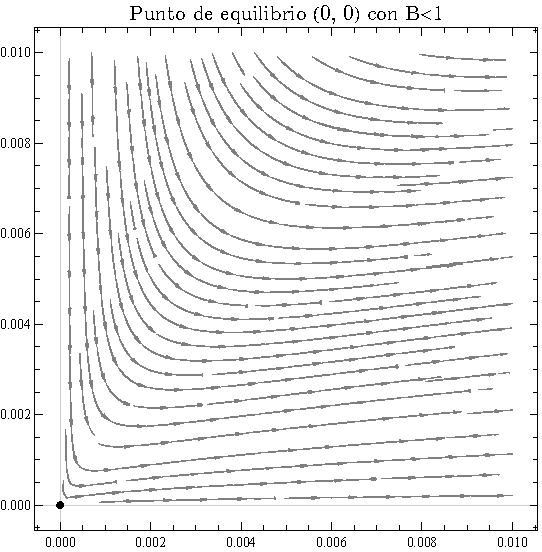
\includegraphics[width=\textwidth]{../img/puntoDeEquilibrio(0,0)conBmenor1.pdf}
			\caption{Retrato fase del sistema \eqref{eq: modelo2} cerca al origen para valores paramétricos aleatorios con $B < 1$.}
			\label{fig: eq(0,0)Modelo2Bmenor1}
		\end{subfigure}
		\begin{subfigure}[t]{0.43\textwidth}
			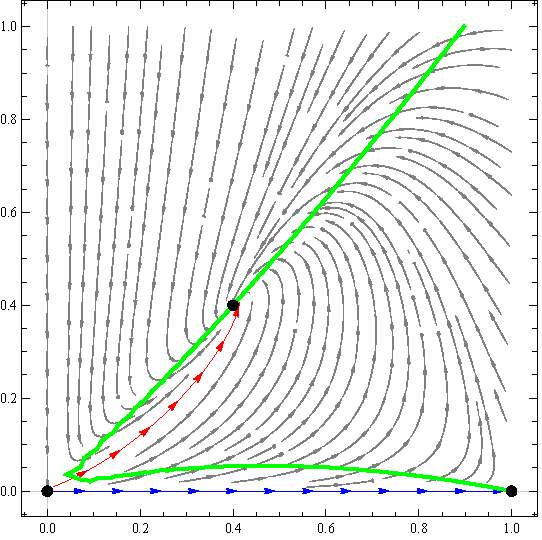
\includegraphics[width=\textwidth]{../img/VariedadesInestablesOrigenBmayor1.pdf}
			\caption{Variedad inestable e isoclina asociada a la pendiente $\dfrac{B-1}{B}$ del sistema \eqref{eq: modelo2}, para $A = 0.05; \; B = 1.5$ y $Q = 0.61$.}
		\end{subfigure}
		\caption{Comportamiento sectorial del primer cuadrante para diferentes valores de B.}
	\end{figure}
	
	\item Se determinó que la estabilidad del punto de equilibrio $(H,H)$ depende de manera fundamental de los valores de los parámetros del sistema. Uno de los principales resultados obtenidos en el \autoref{teo: equilibrioH}, está relacionado con la existencia de ciclos límite y su dependencia respecto de los parámetros del modelo. Además de esto, cuando $B<B_c$, el equilibrio $(H,H)$ es inestable; y, dado que $\Gamma$ es una región positivamente invariante y que los restantes puntos de equilibrio no presentan propiedades atractoras en el interior de la región, el teorema de Poincaré--Bendixson proporciona un mecanismo para establecer la existencia de una órbita periódica bajo las condiciones apropiadas; similarmente, es posible garantizar la existencia de un ciclo límite adicional en el caso donde ocurre una bifurcación de Hopf subcrítica, más sin embargo, a pesar de que las simulaciones numéricas mostradas en la \autoref{fig: simulacionNumericaCiclosAdicionales} validan esta hipotesis, se requiere de una demostración formal. En particular, estos resultados son consistentes con la interpretación biológica de oscilaciones persistentes en las densidades de presa y depredador.
	
	\begin{figure}[H]
		\centering
		\begin{subfigure}[t]{0.46\textwidth}
			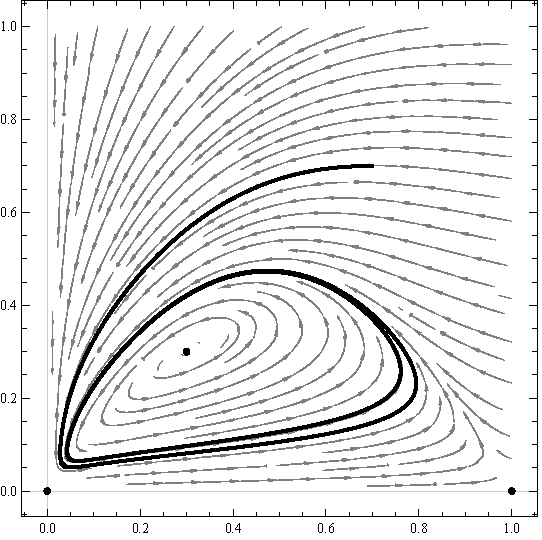
\includegraphics[width=\textwidth]{../img/hFocoInestable.pdf}
			\caption{Retrato fase del sistema \eqref{eq: modelo2} para $A = 0.03; \; B = 0.3$ y $Q = 0.707$ con $(H,H)$ como foco inestable, rodeado por un ciclo límite estable.}
		\end{subfigure}
		\begin{subfigure}[t]{0.46\textwidth}
			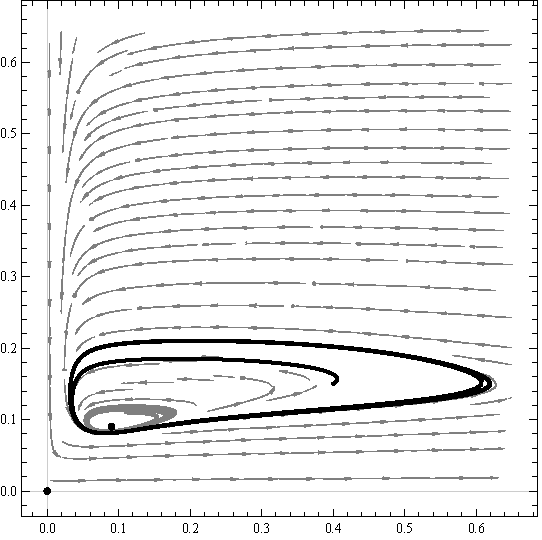
\includegraphics[width=\textwidth]{../img/HopfSubCentrolinealVersion2.pdf}
			\caption{Bifurcación de Hopf subcrítica del sistema \eqref{eq: modelo2} para $A = 0.078; \; B = 0.0643$ y $Q = 1.594$ con $(H,H)$ como foco débil estable, rodeado por un ciclo límite inestable y este a su vez por una orbita periódica estable.}
		\end{subfigure}
		\caption{Orbitas periódicas del modelo de estudio.}
		\label{fig: simulacionNumericaCiclosAdicionales}
	\end{figure}
	
	Por otra parte, en el punto de Bautin $(A_c,B_c)$ se identificó la presencia de dos ciclos límite, uno estable y otro inestable. Esta configuración plantea la posibilidad de que, ante una variación adicional de los parámetros, ambos ciclos límite colisionen y den lugar a un ciclo límite semiestable. Este fenómeno corresponde a una bifurcación de ciclos límite \cite[p.  ~101]{kuznetsov} y constituye una extensión natural del análisis realizado.
\end{enumerate}

\noindent Desde el punto de vista biológico, los resultados obtenidos muestran que la dinámica a largo plazo de las poblaciones depende tanto de las condiciones iniciales como de los valores de los parámetros. En particular, dentro de la región biológicamente relevante, la extinción simultánea de ambas especies únicamente puede ocurrir cuando las condiciones iniciales se encuentran sobre el semieje positivo $u=0$, correspondiente a la ausencia inicial de presas. Por otro lado, en ausencia de depredadores, es decir, cuando las condiciones iniciales pertenecen al semieje positivo $v=0$, la dinámica conduce al equilibrio $(1,0)$, que representa el crecimiento de la población de presas hasta el nivel determinado por la capacidad de carga del ambiente. \\

\noindent Cuando ambas poblaciones están inicialmente presentes, es decir, cuando las condiciones iniciales no se encuentren en los semiejes positivos $u=0$ y $v=0$, los resultados obtenidos indican que la dinámica puede conducir al equilibrio de coexistencia $(H,H)$ o a una órbita periódica, dependiendo de los valores de los parámetros y de las condiciones iniciales. Además, cuando $(H,H)$ es un foco débil estable, la convergencia hacia dicho equilibrio puede ser particularmente lenta. Este fenómeno es aún más pronunciado cuando el equilibrio corresponde a un foco débil de segundo orden, como ocurre en el punto de Bautin. \\

\noindent Los resultados anteriores permiten concluir que, para condiciones iniciales biológicamente factibles en las que ambas especies están presentes, el modelo estudiado no predice la extinción de ambas poblaciones. En su lugar, la dinámica conduce hacia un estado de coexistencia estacionario o hacia oscilaciones persistentes representadas por un ciclo límite. Esto resalta la importancia del análisis cualitativo realizado, pues permite identificar no solo los estados de equilibrio del sistema, sino también las estructuras dinámicas responsables de la persistencia o de las oscilaciones de las poblaciones. \\

\begin{thebibliography}{99}
	
	\bibitem{articulo}
	González-Olivares, E., Tintinago-Ruiz, P.~C., y Rojas-Palma, A. (2015).
	\newblock A {L}eslie--{G}ower-type predator--prey model with sigmoid functional response.
	\newblock \emph{International Journal of Computer Mathematics}, 92(9).
	
	\bibitem{dumortier}
	Dumortier, F., Llibre, J., y Artés, J.~C. (2006).
	\newblock \emph{Qualitative Theory of Planar Differential Systems}.
	\newblock Universitext, Springer-Verlag, Berlin Heidelberg.
	
	\bibitem{kuznetsov}
	Kuznetsov, Yu.~A. (2023).
	\newblock \emph{Elements of Applied Bifurcation Theory}.
	\newblock 4th edition, Applied Mathematical Sciences, Vol. 112, Springer Nature Switzerland AG.
	
	\bibitem{leslie}
	Leslie, P.~H. (1948).
	\newblock Some further notes on the use of matrices in population mathematics.
	\newblock \emph{Biometrika}, 35(3/4).
	
	\bibitem{murray}
	Murray, J.~D. (2002).
	\newblock \emph{Mathematical Biology I: An Introduction}.
	\newblock 3rd edition, Springer-Verlag, New York.
	
	\bibitem{chicone}
	Chicone, C. (2006).
	\newblock \emph{Ordinary Differential Equations with Applications}.
	\newblock 2nd edition, Texts in Applied Mathematics, Vol. 34, Springer, Cham.
	
	\bibitem{perko}
	Perko, L. (2001).
	\newblock \emph{Differential Equations and Dynamical Systems}.
	\newblock 3rd edition, Texts in Applied Mathematics, Vol. 7, Springer-Verlag, New York.

\end{thebibliography}

\end{document}